\def\difficulty{3}
\sujet{Boolean Models}

\index{Spatial Processes!Boolean Models}

\vspace*{-15pt}

\begin{note}This tutorial aims to study a classical model coming from stochastic geometry: the Boolean model. The first objective is to simulate some realizations of a Boolean model of 2-D disks representing a population of overlapped particles. Thereafter, the geometrical characteristics of the individual disks (from a statistical point of view) will be analyzed.  
\end{note}

\vspace*{-10pt}

\begin{figure}[H]
\centering%
\caption{Illustration of 2-D Boolean models observed in a squared window $W$.}%
\subfloat[Boolean model of disks]{
\scalebox{0.75}{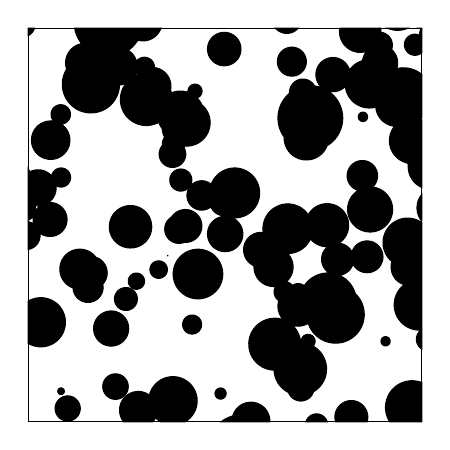
\begin{tikzpicture}[scale=0.01]
\draw[] (0,0) -- (0,500) -- (500,500) -- (500,0) -- (0,0);
\draw[fill=black] (481.3677,499.6506) -- (478.3869,498.6042) -- (475.3165,497.8606) -- (472.1873,497.4272) -- (469.0304,497.3084) -- (465.8774,497.5054) -- (462.7598,498.0161) -- (459.7088,498.8356) -- (456.7549,499.9555) -- (456.6656,500) -- (482.1146,500) -- (481.3677,499.6506);
\draw[fill=black] (342.0925,499.0373) -- (340.684,497.7573) -- (339.1548,496.6244) -- (337.5201,495.6498) -- (335.7963,494.8433) -- (334.0006,494.2129) -- (332.1509,493.765) -- (330.2657,493.5039) -- (328.3639,493.4323) -- (326.4644,493.551) -- (324.5863,493.8587) -- (322.7483,494.3523) -- (320.9687,495.027) -- (319.2654,495.876) -- (317.6553,496.8908) -- (316.1546,498.0612) -- (314.7783,499.3757) -- (314.2434,500) -- (342.9597,500) -- (342.0925,499.0373);
\draw[fill=black] (500,499.6528) -- (500,477.6705) -- (500,468.7559) -- (499.911,468.6751) -- (498.837,467.8794) -- (497.6889,467.1949) -- (496.4782,466.6284) -- (495.217,466.1857) -- (493.9178,465.8711) -- (492.5938,465.6877) -- (491.2581,465.6374) -- (489.924,465.7208) -- (488.6049,465.9369) -- (487.314,466.2836) -- (486.0642,466.7575) -- (484.8679,467.3537) -- (483.7371,468.0665) -- (482.6831,468.8885) -- (481.7164,469.8117) -- (480.8467,470.8268) -- (480.0827,471.9236) -- (479.4321,473.0912) -- (478.9012,474.3179) -- (478.4955,475.5915) -- (478.2189,476.8993) -- (478.0743,478.2281) -- (478.063,479.5647) -- (478.1853,480.8958) -- (478.4398,482.208) -- (478.8241,483.4882) -- (479.3343,484.7237) -- (479.9652,485.9021) -- (480.7106,487.0116) -- (481.5631,488.0412) -- (482.5141,488.9805) -- (483.5542,489.8201) -- (484.6728,490.5518) -- (485.8589,491.1681) -- (487.1006,491.6629) -- (488.3855,492.0312) -- (489.7008,492.2695) -- (491.0333,492.3753) -- (492.3697,492.3475) -- (493.6966,492.1864) -- (495.0008,491.8936) -- (496.2693,491.4722) -- (497.1923,491.0591) -- (497.1914,491.1656) -- (497.4502,493.9826) -- (497.9889,496.7597) -- (498.8021,499.4691) -- (498.9629,499.8586) -- (498.4365,500) -- (500,500) -- (500,499.6528);
\draw[fill=black] (7.5857,498.9375) -- (6.9065,497.4689) -- (6.0841,496.0755) -- (5.1267,494.7712) -- (4.0438,493.5689) -- (2.8464,492.4808) -- (1.5463,491.5176) -- (0.15654,490.689) -- (0,490.6158) -- (0,500) -- (7.9534,500) -- (7.5857,498.9375);
\draw[fill=black] (168.3214,499.0958) -- (167.3054,496.899) -- (166.0751,494.8146) -- (164.6429,492.8634) -- (163.0231,491.0649) -- (161.2318,489.4371) -- (159.287,487.9963) -- (157.208,486.7569) -- (155.0157,485.7312) -- (152.732,484.9294) -- (150.3796,484.3597) -- (147.9821,484.0277) -- (145.5634,483.9367) -- (143.1477,484.0876) -- (140.7591,484.4789) -- (139.2638,484.8805) -- (138.5005,483.5873) -- (135.9149,480.0648) -- (132.9906,476.8179) -- (129.7567,473.8792) -- (127.0422,471.8682) -- (127.5748,471.5628) -- (129.5033,470.1836) -- (131.2846,468.6188) -- (132.9007,466.884) -- (134.3356,464.9965) -- (135.5749,462.9752) -- (136.6062,460.8403) -- (137.4192,458.6131) -- (137.5482,458.108) -- (138.2489,458.9542) -- (139.1552,459.8494) -- (140.1463,460.6495) -- (141.2123,461.3468) -- (142.3427,461.9341) -- (143.526,462.4056) -- (144.7505,462.7567) -- (146.0039,462.9837) -- (147.2737,463.0845) -- (148.5472,463.058) -- (149.8118,462.9045) -- (151.0547,462.6256) -- (152.2635,462.2239) -- (153.4262,461.7036) -- (154.5311,461.0698) -- (155.5673,460.3288) -- (156.5242,459.4881) -- (157.3925,458.5561) -- (158.1634,457.542) -- (158.8292,456.456) -- (159.3833,455.309) -- (159.8201,454.1125) -- (160.1352,452.8783) -- (160.3256,451.6187) -- (160.3892,450.3465) -- (160.371,449.9082) -- (161.6284,449.7556) -- (163.9395,449.2368) -- (166.1874,448.4899) -- (168.3494,447.5224) -- (170.4041,446.3438) -- (172.3308,444.9659) -- (174.1103,443.4027) -- (175.7249,441.6695) -- (177.1584,439.7839) -- (178.3965,437.7645) -- (179.4268,435.6316) -- (180.239,433.4066) -- (180.825,431.1115) -- (181.179,428.7695) -- (181.2973,426.4037) -- (181.2154,424.4348) -- (180.9009,422.0871) -- (180.7673,421.5246) -- (181.6352,419.1468) -- (181.9911,417.7531) -- (184.0478,418.5726) -- (186.8897,419.3874) -- (189.7986,419.9143) -- (192.7457,420.1482) -- (195.7013,420.0867) -- (198.6361,419.7305) -- (201.5206,419.083) -- (203.1687,418.5354) -- (203.1464,418.6407) -- (203.0502,419.5248) -- (203.0427,420.414) -- (203.1241,421.2995) -- (203.2934,422.1725) -- (203.549,423.0242) -- (203.8884,423.8461) -- (204.3082,424.63) -- (204.8041,425.3681) -- (205.3712,426.0531) -- (206.0039,426.6779) -- (206.6958,427.2365) -- (207.44,427.7233) -- (208.2291,428.1333) -- (209.0551,428.4625) -- (209.9099,428.7075) -- (210.7849,428.866) -- (211.6714,428.9364) -- (212.5604,428.9179) -- (213.4432,428.8107) -- (214.3108,428.616) -- (215.1547,428.3356) -- (215.9664,427.9723) -- (216.7377,427.5299) -- (217.461,427.0126) -- (218.1291,426.4257) -- (218.7353,425.7751) -- (219.2734,425.0672) -- (219.7382,424.3091) -- (220.125,423.5084) -- (220.4299,422.6731) -- (220.6499,421.8115) -- (220.7828,420.9322) -- (220.8272,420.0441) -- (220.7965,419.3049) -- (220.6784,418.4235) -- (220.4729,417.5584) -- (220.1821,416.718) -- (219.8088,415.9109) -- (219.3568,415.1451) -- (218.8307,414.4283) -- (218.2355,413.7675) -- (217.5774,413.1695) -- (216.8629,412.6401) -- (216.0991,412.1848) -- (215.2937,411.8079) -- (214.476,411.5209) -- (216.2297,409.6384) -- (218.0189,407.285) -- (219.5641,404.7646) -- (220.5488,402.7262) -- (222.0817,401.3795) -- (224.1118,399.2004) -- (225.9142,396.8294) -- (227.4709,394.2904) -- (228.7664,391.6086) -- (229.7876,388.8109) -- (230.5244,385.9252) -- (230.9695,382.9804) -- (231.1184,380.0058) -- (231.0153,377.5302) -- (230.6198,374.5783) -- (229.9316,371.6806) -- (228.9576,368.8662) -- (227.7074,366.163) -- (226.1936,363.5981) -- (224.4313,361.1972) -- (222.4382,358.9842) -- (220.234,356.9813) -- (217.8409,355.2084) -- (215.2828,353.6833) -- (212.5852,352.4211) -- (209.775,351.4346) -- (206.8804,350.7336) -- (203.9303,350.3251) -- (200.9542,350.2131) -- (198.7725,350.3494) -- (198.7343,350.0646) -- (198.4039,348.6736) -- (198.1589,347.9657) -- (198.8195,346.5983) -- (199.3981,345.0132) -- (199.8156,343.3782) -- (200.0678,341.7097) -- (200.1521,340.0243) -- (200.0937,338.6217) -- (199.8696,336.9492) -- (199.4797,335.3074) -- (198.9278,333.7128) -- (198.2195,332.1812) -- (197.3618,330.728) -- (196.3633,329.3676) -- (195.234,328.1138) -- (193.9852,326.9789) -- (192.6293,325.9744) -- (191.1799,325.1103) -- (189.6514,324.3952) -- (188.0592,323.8363) -- (186.4192,323.4391) -- (184.7477,323.2076) -- (183.0615,323.1442) -- (181.3773,323.2494) -- (179.7121,323.5222) -- (178.0824,323.9599) -- (176.5045,324.5581) -- (174.9943,325.3109) -- (173.5667,326.2106) -- (172.2361,327.2484) -- (171.0158,328.4138) -- (169.9179,329.6953) -- (168.9534,331.0799) -- (168.132,332.5539) -- (167.4618,334.1026) -- (166.9496,335.7104) -- (166.6005,337.3614) -- (166.4179,339.0389) -- (166.4037,340.7263) -- (166.5581,342.4067) -- (166.8794,344.0632) -- (167.3645,345.6794) -- (168.0085,347.2392) -- (168.805,348.7268) -- (169.7461,350.1275) -- (170.4824,351.0167) -- (170.3934,351.835) -- (170.3813,353.2646) -- (170.5121,354.6883) -- (170.7843,356.0917) -- (171.1953,357.461) -- (171.741,358.7825) -- (172.4158,360.0428) -- (173.2131,361.2295) -- (173.3915,361.445) -- (172.7097,362.6685) -- (171.7924,364.7884) -- (171.0912,366.9893) -- (170.6133,369.2492) -- (170.3634,371.5455) -- (170.3568,372.3252) -- (170.2161,372.4895) -- (168.5264,374.9153) -- (167.0873,377.4977) -- (165.9132,380.2109) -- (165.8539,380.3969) -- (165.5631,380.2236) -- (162.574,378.8251) -- (159.4602,377.732) -- (156.2529,376.9552) -- (152.984,376.5025) -- (149.6863,376.3784) -- (146.3926,376.5842) -- (143.136,377.1177) -- (139.9488,377.9737) -- (136.8631,379.1436) -- (133.9096,380.6157) -- (131.1178,382.3754) -- (128.5156,384.4049) -- (126.129,386.6841) -- (123.9819,389.1902) -- (122.0957,391.8981) -- (120.4893,394.7808) -- (119.1786,397.8094) -- (118.1769,400.9538) -- (117.4941,404.1825) -- (117.1371,407.4632) -- (117.1093,410.7631) -- (117.4112,414.0494) -- (118.0396,417.2891) -- (118.9883,420.4498) -- (120.2478,423.5001) -- (121.8055,426.4094) -- (123.6459,429.1486) -- (124.2653,429.8967) -- (123.7245,429.6436) -- (121.4874,428.8583) -- (119.183,428.3002) -- (116.8345,427.975) -- (116.8273,427.9747) -- (116.5137,427.7877) -- (115.9301,427.5147) -- (115.8551,425.711) -- (115.3726,422.11) -- (114.5331,418.5751) -- (113.3448,415.1418) -- (111.8198,411.8442) -- (109.9731,408.7153) -- (107.8233,405.7865) -- (105.3918,403.0869) -- (102.703,400.6435) -- (99.7837,398.4807) -- (96.663,396.6202) -- (93.3722,395.0806) -- (89.9442,393.8772) -- (86.4131,393.022) -- (82.8143,392.5236) -- (79.1837,392.387) -- (75.5576,392.6135) -- (71.9722,393.2009) -- (68.4634,394.1433) -- (65.0662,395.4313) -- (61.8145,397.052) -- (58.741,398.9892) -- (55.8761,401.2236) -- (53.2486,403.7329) -- (50.8848,406.4919) -- (48.8082,409.4731) -- (47.0397,412.6468) -- (45.5968,415.9811) -- (44.4939,419.4429) -- (43.7422,422.9974) -- (43.3491,426.6093) -- (43.3186,430.2423) -- (43.6509,433.8602) -- (44.3427,437.4269) -- (45.3872,440.9067) -- (46.7738,444.2649) -- (48.4888,447.4678) -- (48.843,447.995) -- (48.3229,449.6274) -- (47.8102,452.0517) -- (47.5421,454.5151) -- (47.5213,456.993) -- (47.748,459.4605) -- (48.2198,461.8931) -- (48.9322,464.2664) -- (49.8779,466.5567) -- (51.0475,468.7412) -- (52.4294,470.798) -- (54.0098,472.7066) -- (55.7727,474.4479) -- (57.7007,476.0044) -- (59.7745,477.3607) -- (61.9733,478.5032) -- (64.2752,479.4205) -- (66.6572,480.1034) -- (67.9307,480.3341) -- (67.4346,480.9132) -- (64.9371,484.4988) -- (62.81,488.3157) -- (61.0746,492.326) -- (59.7482,496.4895) -- (59.0058,500) -- (168.6343,500) -- (168.3214,499.0958);
\draw[fill=black] (250.5693,494.7286) -- (252.6764,494.4728) -- (254.7474,494.0079) -- (256.7617,493.3387) -- (258.6991,492.4716) -- (260.5402,491.4155) -- (262.2668,490.1808) -- (263.8614,488.78) -- (265.3082,487.2269) -- (266.5927,485.5372) -- (267.7022,483.7277) -- (268.6254,481.8164) -- (269.3532,479.8226) -- (269.8784,477.766) -- (270.1955,475.6673) -- (270.3016,473.5474) -- (270.2282,471.783) -- (269.9463,469.6793) -- (269.4559,467.6142) -- (268.7617,465.6083) -- (267.8707,463.6818) -- (266.7919,461.8539) -- (265.5359,460.1428) -- (264.1154,458.5657) -- (262.5446,457.1382) -- (260.839,455.8747) -- (259.0159,454.7878) -- (257.0934,453.8883) -- (255.0906,453.1852) -- (253.0277,452.6856) -- (250.9252,452.3944) -- (248.8042,452.3146) -- (246.6858,452.447) -- (244.5911,452.7901) -- (242.5412,453.3407) -- (240.5565,454.0932) -- (238.6569,455.04) -- (236.8612,456.1718) -- (235.1875,457.4771) -- (233.6525,458.9431) -- (232.2715,460.555) -- (231.0584,462.2966) -- (230.0251,464.1507) -- (229.1822,466.0987) -- (228.5379,468.1211) -- (228.0987,470.1977) -- (227.8691,472.3078) -- (227.8512,474.4303) -- (228.0454,476.544) -- (228.4496,478.6277) -- (229.0597,480.6606) -- (229.8698,482.6225) -- (230.8718,484.4937) -- (232.0555,486.2556) -- (233.4092,487.8904) -- (234.9193,489.382) -- (236.5708,490.7153) -- (238.3472,491.8771) -- (240.2306,492.8557) -- (242.2024,493.6415) -- (244.2428,494.2264) -- (246.3313,494.6048) -- (248.4472,494.7727) -- (250.5693,494.7286);
\draw[fill=black] (447.9924,498.2622) -- (448.1237,495.6374) -- (448.0914,494.8594) -- (449.0107,494.7478) -- (450.6185,494.387) -- (452.1821,493.8674) -- (453.6861,493.1943) -- (455.1154,492.3745) -- (456.4557,491.416) -- (457.6936,490.3285) -- (458.8168,489.1229) -- (459.814,487.8112) -- (460.6752,486.4064) -- (461.3919,484.9227) -- (461.9569,483.3749) -- (462.3646,481.7784) -- (462.6108,480.1492) -- (462.6932,478.5035) -- (462.6362,477.1338) -- (462.4174,475.5007) -- (462.0366,473.8975) -- (461.6716,472.843) -- (462.6502,471.9833) -- (464.177,470.3444) -- (465.5326,468.5612) -- (466.7033,466.6517) -- (467.6776,464.6348) -- (468.4457,462.5307) -- (468.9998,460.3604) -- (469.3346,458.1456) -- (469.4465,455.9085) -- (469.369,454.0467) -- (469.0716,451.8266) -- (468.554,449.6473) -- (468.1976,448.6174) -- (468.7904,448.7874) -- (472.3172,449.4262) -- (475.8901,449.7098) -- (479.4734,449.6353) -- (483.0314,449.2034) -- (486.5285,448.4184) -- (489.9298,447.2883) -- (493.2013,445.8242) -- (496.3102,444.0409) -- (499.2256,441.956) -- (500,441.2757) -- (500,386.4379) -- (499.6947,386.1605) -- (497.6105,384.6164) -- (498.653,384.27) -- (500,383.6672) -- (500,356.6893) -- (500,351.0647) -- (500,297.6564) -- (497.7359,298.7849) -- (495.2551,300.3485) -- (492.9429,302.1519) -- (490.8222,304.1772) -- (488.9143,306.4041) -- (487.2383,308.8103) -- (485.8108,311.3718) -- (484.6462,314.063) -- (483.7561,316.857) -- (483.1494,319.7259) -- (482.8321,322.6411) -- (482.8075,325.5734) -- (482.9867,327.5251) -- (482.1477,328.1796) -- (481.5461,328.7541) -- (479.1447,329.399) -- (476.422,330.4313) -- (473.816,331.7302) -- (471.3526,333.2828) -- (469.0566,335.0736) -- (466.9508,337.0847) -- (465.0563,339.2959) -- (463.392,341.6852) -- (461.9746,344.2287) -- (460.8182,346.9011) -- (459.9343,349.6755) -- (459.3318,352.5243) -- (459.0168,355.419) -- (458.9923,358.3307) -- (459.2586,361.2303) -- (459.8131,364.0889) -- (460.6502,366.8778) -- (461.7615,369.5692) -- (463.136,372.1362) -- (464.7599,374.5531) -- (465.4658,375.4057) -- (465.3652,375.412) -- (462.7144,375.8463) -- (460.1203,376.543) -- (457.6087,377.4953) -- (455.2047,378.6935) -- (452.9323,380.1258) -- (450.8142,381.7777) -- (448.8717,383.6328) -- (447.1241,385.6726) -- (445.5888,387.8767) -- (444.2813,390.2231) -- (443.2145,392.6882) -- (442.3992,395.2476) -- (441.8434,397.8755) -- (441.6384,399.759) -- (439.2232,399.1741) -- (436.1818,398.7529) -- (433.1136,398.6374) -- (430.0491,398.8288) -- (427.0191,399.3253) -- (424.0538,400.1217) -- (421.1827,401.2102) -- (418.4348,402.5799) -- (415.8372,404.217) -- (413.4161,406.1054) -- (411.1956,408.2259) -- (409.1979,410.5576) -- (407.443,413.0771) -- (405.9484,415.7592) -- (404.7289,418.5771) -- (403.7969,421.5026) -- (403.1617,424.5066) -- (402.9851,426.129) -- (402.6404,425.7464) -- (401.0347,424.2872) -- (399.2913,422.9956) -- (397.4277,421.8846) -- (395.4624,420.9651) -- (393.4152,420.2464) -- (391.3065,419.7357) -- (389.1573,419.4381) -- (386.9892,419.3565) -- (384.8237,419.4918) -- (382.6826,419.8426) -- (380.9792,420.3001) -- (384.0705,418.0894) -- (387.1608,415.3747) -- (389.9645,412.3651) -- (392.4538,409.0906) -- (394.6038,405.5839) -- (396.3929,401.8801) -- (397.8034,398.0162) -- (398.821,394.0308) -- (399.4357,389.9637) -- (399.6413,385.8556) -- (399.499,382.4365) -- (398.9527,378.3596) -- (398.0023,374.3577) -- (396.657,370.4706) -- (394.9304,366.7373) -- (392.8397,363.1949) -- (390.4058,359.879) -- (387.653,356.8227) -- (384.6089,354.0564) -- (381.3038,351.6079) -- (379.7464,350.6793) -- (379.6179,350.3081) -- (378.4319,347.7437) -- (376.9957,345.3104) -- (375.3239,343.0327) -- (373.433,340.9332) -- (371.3419,339.0331) -- (369.0716,337.3511) -- (366.6447,335.9043) -- (364.0855,334.7069) -- (361.4196,333.771) -- (358.6735,333.106) -- (355.8748,332.7184) -- (353.0513,332.6121) -- (350.2314,332.7883) -- (347.4431,333.2451) -- (344.7143,333.978) -- (342.0724,334.9796) -- (339.5436,336.24) -- (337.1534,337.7466) -- (334.9254,339.4843) -- (332.8821,341.4357) -- (331.0438,343.5813) -- (329.4289,345.8998) -- (328.0535,348.3678) -- (326.9313,350.9609) -- (326.0737,353.6531) -- (325.4891,356.4174) -- (325.1834,359.2262) -- (325.1618,361.7994) -- (323.5921,364.0529) -- (321.5898,367.6459) -- (319.9563,371.4209) -- (318.7077,375.3401) -- (317.8567,379.3644) -- (317.4116,383.4535) -- (317.377,387.5666) -- (317.7533,391.6627) -- (318.5365,395.7007) -- (319.719,399.6403) -- (321.2889,403.4422) -- (323.2305,407.0684) -- (325.5244,410.4827) -- (328.1477,413.6508) -- (331.0742,416.5413) -- (332.0451,417.3252) -- (332.0323,417.4429) -- (332.0181,419.1376) -- (332.1731,420.8254) -- (332.4958,422.4892) -- (332.983,424.1125) -- (333.6299,425.679) -- (334.4299,427.1732) -- (335.3751,428.58) -- (336.456,429.8854) -- (337.6618,431.0764) -- (338.9806,432.1411) -- (340.399,433.0687) -- (341.9029,433.8502) -- (343.4773,434.4776) -- (345.1065,434.9447) -- (346.7742,435.2468) -- (348.4638,435.3809) -- (350.1582,435.3456) -- (351.8407,435.1414) -- (353.4944,434.7702) -- (355.1028,434.2358) -- (356.6498,433.5435) -- (358.1199,432.7002) -- (359.4986,431.7143) -- (360.7719,430.5957) -- (361.9271,429.3556) -- (362.9528,428.0064) -- (363.8088,426.6103) -- (365.4855,426.4067) -- (369.4989,425.5059) -- (373.4023,424.2089) -- (373.9007,423.9859) -- (373.0701,424.6337) -- (371.5011,426.1322) -- (370.0894,427.7798) -- (368.8493,429.5602) -- (367.7931,431.4555) -- (366.9314,433.4467) -- (366.2728,435.514) -- (365.8239,437.6368) -- (365.5892,439.7937) -- (365.5709,441.9633) -- (365.7694,444.1239) -- (366.1825,446.2539) -- (366.8063,448.332) -- (367.6344,450.3374) -- (368.6585,452.2502) -- (369.8685,454.0512) -- (371.2523,455.7223) -- (372.7959,457.247) -- (374.4841,458.6099) -- (376.2999,459.7975) -- (378.2252,460.7979) -- (380.2408,461.6011) -- (382.3265,462.199) -- (384.4614,462.5858) -- (386.6243,462.7574) -- (388.7935,462.7123) -- (390.9474,462.4509) -- (393.0644,461.9757) -- (395.1234,461.2915) -- (397.1038,460.4053) -- (398.9859,459.3257) -- (400.7507,458.0636) -- (402.3808,456.6317) -- (403.8597,455.0441) -- (405.1728,453.3169) -- (406.3068,451.4671) -- (407.2506,449.5135) -- (407.9946,447.4753) -- (408.1918,446.703) -- (408.8854,447.7354) -- (410.8436,450.1003) -- (413.0281,452.2579) -- (415.4171,454.1867) -- (417.9867,455.8673) -- (420.7113,457.283) -- (423.5636,458.4196) -- (424.8275,458.782) -- (424.8541,459.0708) -- (425.2806,461.2697) -- (425.9245,463.4151) -- (426.7794,465.4854) -- (427.8367,467.4601) -- (429.0859,469.3193) -- (430.2936,470.7779) -- (429.29,470.4256) -- (426.7357,469.807) -- (424.1325,469.4465) -- (421.5063,469.3476) -- (418.8833,469.5115) -- (416.2898,469.9364) -- (413.7517,470.6181) -- (411.2943,471.5498) -- (408.9422,472.7221) -- (406.7189,474.1234) -- (404.6465,475.7397) -- (402.746,477.5548) -- (401.0361,479.5506) -- (399.5339,481.707) -- (398.2546,484.0027) -- (397.2109,486.4147) -- (396.4132,488.9187) -- (395.8694,491.49) -- (395.5851,494.1026) -- (395.563,496.7306) -- (395.8033,499.3477) -- (395.9299,500) -- (447.7297,500) -- (447.9924,498.2622);
\draw[fill=black] (336.2811,475.895) -- (338.1081,475.6732) -- (339.9038,475.2701) -- (341.6503,474.6898) -- (343.3301,473.9381) -- (344.9265,473.0223) -- (346.4235,471.9518) -- (347.8062,470.7372) -- (349.0607,469.3906) -- (350.1744,467.9255) -- (351.1364,466.3565) -- (351.9369,464.6993) -- (352.568,462.9705) -- (353.0233,461.1873) -- (353.2983,459.3676) -- (353.3903,457.5295) -- (353.3266,455.9997) -- (353.0822,454.1756) -- (352.657,452.385) -- (352.0551,450.6458) -- (351.2825,448.9754) -- (350.3471,447.3905) -- (349.2581,445.9069) -- (348.0264,444.5394) -- (346.6644,443.3017) -- (345.1856,442.2061) -- (343.6048,441.2637) -- (341.9379,440.4838) -- (340.2014,439.8742) -- (338.4127,439.441) -- (336.5897,439.1885) -- (334.7506,439.1193) -- (332.9138,439.2341) -- (331.0976,439.5316) -- (329.3202,440.009) -- (327.5993,440.6614) -- (325.9522,441.4824) -- (324.3953,442.4637) -- (322.9441,443.5956) -- (321.6131,444.8666) -- (320.4157,446.2642) -- (319.3638,447.7744) -- (318.4679,449.382) -- (317.737,451.071) -- (317.1784,452.8246) -- (316.7976,454.6252) -- (316.5985,456.4547) -- (316.583,458.2951) -- (316.7514,460.1277) -- (317.1018,461.9345) -- (317.6309,463.6972) -- (318.3333,465.3982) -- (319.202,467.0207) -- (320.2284,468.5483) -- (321.4021,469.9659) -- (322.7115,471.2591) -- (324.1435,472.4152) -- (325.6837,473.4226) -- (327.3168,474.2711) -- (329.0264,474.9524) -- (330.7955,475.4596) -- (332.6065,475.7876) -- (334.4411,475.9333) -- (336.2811,475.895);
\draw[fill=white] (136.9835,443.3858) -- (136.7584,442.7353) -- (135.7632,440.5834) -- (134.558,438.5415) -- (134.4802,438.4355) -- (136.3564,439.4104) -- (138.3644,440.2105) -- (138.6163,440.5855) -- (138.9793,441.0239) -- (138.3949,441.582) -- (137.5662,442.5494) -- (136.9835,443.3858);
\draw[fill=black] (42.2115,402.749) -- (43.4345,402.6006) -- (44.6365,402.3308) -- (45.8056,401.9423) -- (46.9301,401.4391) -- (47.9988,400.8261) -- (49.0008,400.1095) -- (49.9264,399.2964) -- (50.7661,398.395) -- (51.5117,397.4143) -- (52.1556,396.364) -- (52.6915,395.2547) -- (53.1139,394.0974) -- (53.4187,392.9038) -- (53.6028,391.6857) -- (53.6644,390.4553) -- (53.6218,389.4312) -- (53.4582,388.2102) -- (53.1735,387.0116) -- (52.7706,385.8474) -- (52.2534,384.7292) -- (51.6273,383.6682) -- (50.8983,382.6751) -- (50.0738,381.7597) -- (49.1621,380.9312) -- (48.1722,380.1978) -- (47.114,379.567) -- (45.9982,379.0449) -- (44.8358,378.6368) -- (43.6384,378.3469) -- (42.4181,378.1779) -- (41.8835,378.1578) -- (43.6973,376.8607) -- (45.5301,375.2506) -- (47.1931,373.4655) -- (48.6695,371.5234) -- (49.9447,369.4435) -- (51.0059,367.2467) -- (51.8424,364.955) -- (52.446,362.5912) -- (52.8106,360.179) -- (52.9325,357.7424) -- (52.8481,355.7144) -- (52.5241,353.2964) -- (51.9604,350.9228) -- (51.1625,348.6173) -- (50.1384,346.403) -- (48.8984,344.302) -- (47.4548,342.3353) -- (45.8221,340.5226) -- (44.0166,338.8818) -- (42.0563,337.4296) -- (39.9608,336.1803) -- (37.7511,335.1464) -- (35.4491,334.3383) -- (33.0781,333.7641) -- (30.6615,333.4294) -- (28.2236,333.3377) -- (25.7887,333.4898) -- (23.3811,333.8842) -- (21.025,334.517) -- (18.7438,335.3819) -- (16.5603,336.4702) -- (14.4964,337.771) -- (12.5727,339.2714) -- (10.8084,340.9564) -- (9.2211,342.809) -- (7.8267,344.8109) -- (6.6391,346.942) -- (5.6702,349.181) -- (4.9297,351.5055) -- (4.4249,353.8923) -- (4.161,356.3177) -- (4.1405,358.7572) -- (4.3636,361.1866) -- (4.8282,363.5816) -- (5.5295,365.9183) -- (6.4606,368.1732) -- (7.6122,370.324) -- (8.9728,372.349) -- (10.5287,374.2281) -- (12.2644,375.9425) -- (14.1626,377.475) -- (16.2044,378.8103) -- (18.3692,379.9352) -- (20.6355,380.8383) -- (22.9807,381.5107) -- (25.3813,381.9455) -- (27.8133,382.1385) -- (30.2524,382.0878) -- (32.5737,381.806) -- (32.3928,381.9788) -- (31.5913,382.9143) -- (30.8872,383.9252) -- (30.2875,385.0013) -- (29.7982,386.132) -- (29.4243,387.3058) -- (29.1694,388.5111) -- (29.0361,389.7358) -- (29.0257,390.9677) -- (29.1384,392.1945) -- (29.373,393.4039) -- (29.7271,394.5839) -- (30.1973,395.7226) -- (30.7789,396.8086) -- (31.4659,397.8312) -- (32.2516,398.7801) -- (33.1281,399.6458) -- (34.0866,400.4197) -- (35.1177,401.094) -- (36.2108,401.662) -- (37.3553,402.1181) -- (38.5395,402.4576) -- (39.7518,402.6772) -- (40.9798,402.7747) -- (42.2115,402.749);
\draw[fill=black] (425.7326,393.312) -- (426.3197,393.2407) -- (426.8967,393.1112) -- (427.4579,392.9248) -- (427.9977,392.6832) -- (428.5106,392.3889) -- (428.9917,392.045) -- (429.4359,391.6547) -- (429.839,391.222) -- (430.1969,390.7512) -- (430.506,390.2471) -- (430.7632,389.7146) -- (430.966,389.1591) -- (431.1123,388.5861) -- (431.2007,388.0014) -- (431.2302,387.4107) -- (431.2098,386.9192) -- (431.1313,386.333) -- (430.9946,385.7577) -- (430.8012,385.1988) -- (430.553,384.6621) -- (430.2524,384.1528) -- (429.9025,383.6761) -- (429.5067,383.2367) -- (429.0691,382.839) -- (428.5939,382.487) -- (428.0859,382.1841) -- (427.5503,381.9335) -- (426.9923,381.7377) -- (426.4176,381.5985) -- (425.8318,381.5173) -- (425.2409,381.4951) -- (424.6507,381.532) -- (424.0671,381.6276) -- (423.496,381.781) -- (422.943,381.9906) -- (422.4137,382.2544) -- (421.9135,382.5697) -- (421.4471,382.9334) -- (421.0195,383.3418) -- (420.6347,383.7909) -- (420.2967,384.2762) -- (420.0089,384.7927) -- (419.774,385.3355) -- (419.5945,385.8989) -- (419.4721,386.4775) -- (419.4082,387.0654) -- (419.4032,387.6567) -- (419.4573,388.2456) -- (419.5699,388.8262) -- (419.7399,389.3926) -- (419.9656,389.9391) -- (420.2447,390.4605) -- (420.5745,390.9513) -- (420.9517,391.4068) -- (421.3724,391.8224) -- (421.8325,392.1939) -- (422.3274,392.5176) -- (422.8522,392.7902) -- (423.4015,393.0091) -- (423.97,393.1721) -- (424.5519,393.2775) -- (425.1414,393.3243) -- (425.7326,393.312);
\draw[fill=black] (42.6087,322.3598) -- (43.8096,322.2141) -- (44.9898,321.9491) -- (46.1378,321.5677) -- (47.2419,321.0736) -- (48.2911,320.4717) -- (49.2751,319.7681) -- (50.1838,318.9698) -- (51.0084,318.0847) -- (51.7404,317.1217) -- (52.3727,316.0905) -- (52.8989,315.0012) -- (53.3136,313.8649) -- (53.6129,312.6929) -- (53.7937,311.4968) -- (53.8541,310.2887) -- (53.8123,309.2832) -- (53.6517,308.0843) -- (53.3721,306.9074) -- (52.9765,305.7643) -- (52.4688,304.6664) -- (51.8539,303.6246) -- (51.1382,302.6495) -- (50.3286,301.7507) -- (49.4334,300.9372) -- (48.4614,300.2171) -- (47.4224,299.5977) -- (46.3268,299.085) -- (45.1854,298.6844) -- (44.0098,298.3996) -- (42.8116,298.2337) -- (41.6028,298.1882) -- (40.3955,298.2636) -- (39.2018,298.4592) -- (38.0335,298.773) -- (36.9025,299.2018) -- (35.8199,299.7414) -- (35.2597,300.0944) -- (35.3593,299.4357) -- (35.474,297.1447) -- (35.3946,295.2379) -- (35.09,292.9643) -- (34.5599,290.7325) -- (33.8097,288.5648) -- (32.8468,286.4828) -- (31.6809,284.5073) -- (30.3236,282.6581) -- (28.7884,280.9537) -- (27.0907,279.411) -- (25.6719,278.3599) -- (27.1383,278.4763) -- (29.2906,278.4315) -- (31.4276,278.1721) -- (33.5281,277.7006) -- (35.571,277.0218) -- (37.5359,276.1425) -- (39.4032,275.0713) -- (41.1542,273.8191) -- (42.7715,272.3984) -- (44.2389,270.8233) -- (45.5417,269.1095) -- (46.6669,267.2743) -- (47.6032,265.3359) -- (48.3414,263.3137) -- (48.874,261.2279) -- (49.1957,259.0994) -- (49.3033,256.9493) -- (49.2288,255.1599) -- (48.943,253.0263) -- (48.4455,250.9318) -- (47.7415,248.8975) -- (46.8378,246.9436) -- (45.7436,245.0897) -- (44.4698,243.3543) -- (43.0292,241.7548) -- (41.436,240.307) -- (39.7062,239.0256) -- (37.8572,237.9232) -- (35.9074,237.0109) -- (33.8762,236.2979) -- (31.7839,235.7912) -- (29.6516,235.4959) -- (27.5004,235.4149) -- (25.3519,235.5491) -- (23.2275,235.8972) -- (21.1484,236.4556) -- (19.1355,237.2187) -- (17.2089,238.179) -- (15.3877,239.3269) -- (14.6775,239.8808) -- (14.9218,238.2643) -- (15.0105,236.4905) -- (14.9491,235.0143) -- (14.7133,233.2541) -- (14.3029,231.5262) -- (13.7221,229.8479) -- (12.9766,228.236) -- (12.0739,226.7066) -- (11.023,225.2749) -- (9.8345,223.9553) -- (8.5202,222.7609) -- (7.0932,221.7038) -- (5.5678,220.7943) -- (3.9592,220.0417) -- (2.2835,219.4535) -- (0.55743,219.0354) -- (0,218.9582) -- (0,254.0308) -- (0.26347,253.9989) -- (1.9963,253.6099) -- (3.6816,253.0499) -- (5.3027,252.3245) -- (6.8432,251.4408) -- (6.9787,251.3439) -- (6.9461,251.446) -- (6.5007,253.5521) -- (6.2678,255.6922) -- (6.2497,257.8448) -- (6.4466,259.9885) -- (6.8565,262.1018) -- (7.0115,262.6181) -- (6.3456,261.4898) -- (5.3611,260.1486) -- (4.2478,258.9125) -- (3.0166,257.7936) -- (1.6798,256.8033) -- (0.25083,255.9514) -- (0,255.834) -- (0,277.9469) -- (0,297.1652) -- (0,316.3391) -- (0,321.8388) -- (0.036016,321.78) -- (1.151,319.4719) -- (1.89,317.4475) -- (2.9756,318.0116) -- (5.1066,318.8608) -- (7.3116,319.4929) -- (9.5688,319.9018) -- (11.8555,320.0833) -- (14.1489,320.0356) -- (16.426,319.7592) -- (18.6642,319.2568) -- (20.8411,318.5335) -- (22.9349,317.5965) -- (24.9246,316.4551) -- (26.7905,315.1208) -- (28.5139,313.6069) -- (29.814,312.2112) -- (30.0027,313.184) -- (30.3505,314.3426) -- (30.8121,315.4606) -- (31.3831,316.527) -- (32.0577,317.5311) -- (32.8292,318.4628) -- (33.6898,319.3128) -- (34.631,320.0727) -- (35.6434,320.7348) -- (36.7167,321.2925) -- (37.8404,321.7403) -- (39.0032,322.0737) -- (40.1935,322.2893) -- (41.3994,322.385) -- (42.6087,322.3598);
\draw[fill=black] (264.5553,322.3355) -- (267.7056,321.9531) -- (270.802,321.2581) -- (273.8135,320.2574) -- (276.7101,318.9611) -- (279.4628,317.3821) -- (282.0442,315.5362) -- (284.4283,313.4418) -- (286.5914,311.1198) -- (288.512,308.5935) -- (290.1707,305.888) -- (291.551,303.0305) -- (292.6392,300.0495) -- (293.4243,296.9747) -- (293.8985,293.8369) -- (294.0571,290.6674) -- (293.9474,288.0295) -- (293.526,284.8842) -- (292.7927,281.7966) -- (291.7548,278.7977) -- (290.4227,275.9174) -- (288.8097,273.1845) -- (286.9319,270.6262) -- (284.8081,268.2682) -- (282.4595,266.134) -- (279.9096,264.2449) -- (277.1838,262.6198) -- (274.3094,261.275) -- (271.3151,260.2239) -- (268.2309,259.4769) -- (265.0874,259.0416) -- (261.9162,258.9222) -- (259.2133,259.0911) -- (260.4342,258.5447) -- (262.3807,257.4282) -- (264.2059,256.1229) -- (265.8918,254.6419) -- (267.4213,253) -- (268.7793,251.2137) -- (269.9522,249.3007) -- (270.9283,247.2801) -- (271.6977,245.1722) -- (272.2529,242.998) -- (272.5882,240.7792) -- (272.7004,238.5381) -- (272.6227,236.6728) -- (272.3247,234.4488) -- (271.8062,232.2656) -- (271.0723,230.145) -- (270.1304,228.1083) -- (268.9898,226.1759) -- (267.6621,224.3669) -- (266.1603,222.6995) -- (264.4996,221.1904) -- (262.6966,219.8547) -- (260.7692,218.7056) -- (258.7367,217.7546) -- (256.6194,217.0114) -- (254.4385,216.4832) -- (252.2158,216.1754) -- (249.9734,216.091) -- (247.7338,216.2309) -- (245.5194,216.5937) -- (243.3522,217.1757) -- (241.254,217.9712) -- (239.2457,218.9722) -- (237.3474,220.1687) -- (235.578,221.5488) -- (233.9552,223.0986) -- (232.4952,224.8026) -- (231.2127,226.6439) -- (230.1203,228.604) -- (229.2292,230.6634) -- (228.548,232.8015) -- (228.0837,234.9969) -- (227.841,237.2277) -- (227.8221,239.4715) -- (228.0273,241.7061) -- (228.4546,243.909) -- (229.0997,246.0582) -- (229.9561,248.1323) -- (231.0154,250.1105) -- (232.2668,251.9731) -- (233.6979,253.7015) -- (235.2944,255.2783) -- (237.0403,256.6879) -- (238.9183,257.9162) -- (240.9095,258.9508) -- (242.994,259.7814) -- (245.1511,260.3999) -- (247.3591,260.7998) -- (249.596,260.9774) -- (251.27,260.9426) -- (249.5851,261.5813) -- (249.2983,261.7243) -- (248.9744,261.7121) -- (247.1219,261.8278) -- (245.2903,262.1279) -- (243.4977,262.6093) -- (241.7622,263.2673) -- (240.1011,264.0953) -- (238.5309,265.085) -- (237.0673,266.2264) -- (235.725,267.5083) -- (234.5174,268.9178) -- (233.4566,270.4408) -- (232.5531,272.0621) -- (232.128,273.0446) -- (230.7085,271.993) -- (229.1071,271.0383) -- (227.4184,270.2482) -- (225.6593,269.6306) -- (223.8472,269.1918) -- (222.0005,268.936) -- (220.1374,268.8659) -- (218.2766,268.9822) -- (216.4367,269.2836) -- (214.6361,269.7672) -- (212.8928,270.4281) -- (211.2242,271.2598) -- (209.6469,272.2539) -- (208.1768,273.4006) -- (206.8285,274.6882) -- (205.6155,276.104) -- (204.5498,277.6339) -- (203.6423,279.2625) -- (202.9018,280.9735) -- (202.3359,282.75) -- (201.9502,284.574) -- (201.7484,286.4275) -- (201.7328,288.2918) -- (201.9033,290.1484) -- (202.2583,291.9787) -- (202.7943,293.7644) -- (203.5059,295.4877) -- (204.3859,297.1313) -- (205.4257,298.6789) -- (206.6147,300.1149) -- (207.9412,301.425) -- (209.3918,302.5962) -- (210.9521,303.6167) -- (212.6065,304.4763) -- (214.3385,305.1665) -- (216.1307,305.6803) -- (217.9653,306.0126) -- (219.8238,306.1602) -- (221.6878,306.1214) -- (223.5386,305.8967) -- (225.3578,305.4884) -- (227.1271,304.9005) -- (228.8288,304.1389) -- (230.4461,303.2113) -- (231.9626,302.1268) -- (232.5306,301.6278) -- (233.6074,304.2357) -- (235.1054,307.0334) -- (236.8751,309.6675) -- (238.899,312.1118) -- (241.1569,314.3418) -- (243.626,316.3353) -- (246.2819,318.0723) -- (249.0979,319.5354) -- (252.0459,320.7102) -- (255.0964,321.5848) -- (258.219,322.1504) -- (261.3825,322.4015) -- (264.5553,322.3355);
\draw[fill=black] (194.8747,321.0444) -- (196.2642,320.8757) -- (197.6299,320.5692) -- (198.9581,320.1278) -- (200.2357,319.5561) -- (201.4498,318.8597) -- (202.5883,318.0455) -- (203.6398,317.1218) -- (204.5939,316.0976) -- (205.441,314.9834) -- (206.1726,313.7901) -- (206.7814,312.5298) -- (207.2613,311.215) -- (207.6076,309.8588) -- (207.8167,308.4749) -- (207.8867,307.077) -- (207.8383,305.9135) -- (207.6524,304.5262) -- (207.329,303.1645) -- (206.8712,301.8418) -- (206.2837,300.5714) -- (205.5723,299.366) -- (204.7441,298.2377) -- (203.8074,297.1977) -- (202.7715,296.2563) -- (201.6468,295.4232) -- (200.4446,294.7064) -- (199.1768,294.1133) -- (197.8562,293.6496) -- (196.4958,293.3202) -- (195.1094,293.1282) -- (193.7107,293.0756) -- (192.3138,293.1628) -- (190.9325,293.3891) -- (189.5808,293.7522) -- (188.272,294.2484) -- (187.0193,294.8727) -- (185.8352,295.6191) -- (184.7316,296.4799) -- (183.7193,297.4465) -- (182.8087,298.5094) -- (182.0087,299.6579) -- (181.3274,300.8806) -- (180.7715,302.1651) -- (180.3466,303.4988) -- (180.057,304.8681) -- (179.9056,306.2596) -- (179.8938,307.6592) -- (180.0218,309.053) -- (180.2884,310.4271) -- (180.6907,311.7676) -- (181.2249,313.0614) -- (181.8856,314.2953) -- (182.6662,315.4571) -- (183.5589,316.5351) -- (184.5547,317.5187) -- (185.6437,318.3979) -- (186.8151,319.1641) -- (188.0571,319.8094) -- (189.3573,320.3275) -- (190.7028,320.7133) -- (192.0801,320.9628) -- (193.4753,321.0735) -- (194.8747,321.0444);
\draw[fill=white] (8.6118,274.5606) -- (8.7647,273.9615) -- (9.0133,272.3166) -- (9.0965,270.655) -- (9.0389,269.2721) -- (8.818,267.6232) -- (8.606,266.7305) -- (9.3132,268.0512) -- (10.5137,269.8381) -- (11.8866,271.4962) -- (13.4182,273.0089) -- (15.0932,274.3612) -- (15.0943,274.362) -- (14.5335,274.2843) -- (12.2413,274.198) -- (9.9518,274.3411) -- (8.6118,274.5606);
\draw[fill=black] (381.7212,276.9983) -- (384.4379,276.6685) -- (387.1081,276.0692) -- (389.7051,275.2063) -- (392.2031,274.0884) -- (394.5769,272.7267) -- (396.8029,271.1349) -- (398.8589,269.3287) -- (400.7243,267.3263) -- (402.3805,265.1477) -- (403.8109,262.8147) -- (405.0012,260.3505) -- (405.9396,257.7798) -- (406.6167,255.1282) -- (407.0256,252.4223) -- (407.1624,249.6891) -- (407.0677,247.4143) -- (406.7043,244.7019) -- (406.072,242.0393) -- (405.1769,239.4531) -- (404.0282,236.9693) -- (402.6372,234.6125) -- (401.0179,232.4064) -- (399.1864,230.3729) -- (397.1611,228.5325) -- (394.9621,226.9034) -- (394.7085,226.7522) -- (396.6327,226.5186) -- (398.6225,226.072) -- (400.5577,225.4289) -- (402.4191,224.5959) -- (404.1881,223.5812) -- (405.8468,222.395) -- (407.3789,221.0491) -- (408.769,219.557) -- (410.0031,217.9335) -- (411.0691,216.195) -- (411.3568,215.5993) -- (411.5577,216.2687) -- (412.3278,218.1337) -- (413.2802,219.9124) -- (414.4054,221.5872) -- (415.6922,223.1412) -- (417.1277,224.5591) -- (418.6976,225.8265) -- (420.3862,226.9309) -- (422.1766,227.8612) -- (424.0509,228.6081) -- (425.9905,229.1642) -- (427.9758,229.5238) -- (429.9872,229.6835) -- (432.0044,229.6415) -- (434.0074,229.3984) -- (435.9761,228.9565) -- (437.8908,228.3203) -- (439.7325,227.4961) -- (441.4827,226.4921) -- (443.1239,225.3185) -- (444.6397,223.9869) -- (446.015,222.5106) -- (447.2361,220.9043) -- (448.2907,219.1842) -- (449.1683,217.3674) -- (449.8602,215.4721) -- (450.3594,213.5171) -- (450.6609,211.5221) -- (450.7617,209.5069) -- (450.6919,207.8298) -- (450.424,205.83) -- (449.9577,203.8669) -- (449.2979,201.9602) -- (448.4509,200.1289) -- (447.4254,198.3913) -- (446.2315,196.7647) -- (444.8812,195.2655) -- (443.3879,193.9086) -- (441.7667,192.7075) -- (440.0337,191.6743) -- (438.2061,190.8193) -- (436.3023,190.1509) -- (434.3414,189.676) -- (432.3428,189.3992) -- (430.3265,189.3234) -- (428.3128,189.4492) -- (426.3216,189.7754) -- (424.373,190.2987) -- (422.4864,191.014) -- (420.6806,191.9141) -- (418.9737,192.9899) -- (417.3827,194.2308) -- (415.9235,195.6243) -- (414.6108,197.1565) -- (413.4576,198.8121) -- (412.6176,200.3195) -- (412.087,198.7864) -- (411.231,196.9355) -- (410.1944,195.1792) -- (408.9878,193.5353) -- (407.623,192.02) -- (406.1138,190.6485) -- (404.4751,189.4346) -- (402.7235,188.3903) -- (400.8764,187.5261) -- (398.9522,186.8506) -- (396.9702,186.3706) -- (394.9502,186.0908) -- (394.92,186.0897) -- (397.2341,185.054) -- (400.3678,183.2565) -- (403.3063,181.1551) -- (406.0204,178.7709) -- (408.4829,176.1276) -- (410.6692,173.2517) -- (412.5574,170.1718) -- (414.1288,166.9189) -- (415.3675,163.5253) -- (415.562,162.7636) -- (415.9212,162.4481) -- (418.4065,159.7803) -- (420.6131,156.8777) -- (422.5189,153.7693) -- (424.1048,150.4861) -- (425.355,147.0611) -- (426.2571,143.5283) -- (426.802,139.9232) -- (426.9842,136.2816) -- (426.8581,133.2508) -- (426.3739,129.637) -- (425.5314,126.0896) -- (424.3389,122.644) -- (422.8084,119.3347) -- (420.9551,116.1947) -- (418.7977,113.2554) -- (416.3576,110.5461) -- (413.6592,108.0941) -- (410.7294,105.9236) -- (407.5977,104.0565) -- (404.2952,102.5114) -- (400.8549,101.3036) -- (397.3112,100.4454) -- (393.6996,99.9453) -- (390.0561,99.8082) -- (386.417,100.0355) -- (382.8189,100.625) -- (379.2976,101.5707) -- (375.8883,102.8633) -- (372.6251,104.4898) -- (369.5405,106.4339) -- (366.6655,108.6763) -- (364.0287,111.1945) -- (361.6564,113.9633) -- (359.5724,116.9552) -- (357.7976,120.1401) -- (356.3495,123.4864) -- (355.8507,125.0523) -- (354.6981,124.3651) -- (352.3935,123.2869) -- (349.9928,122.4441) -- (347.5199,121.8452) -- (344.9997,121.4962) -- (342.4571,121.4005) -- (339.9177,121.5592) -- (337.4068,121.9705) -- (335.9784,122.3542) -- (336.1803,122.1768) -- (338.4266,119.7656) -- (340.4209,117.1422) -- (342.1433,114.3329) -- (343.5767,111.3656) -- (344.7066,108.2701) -- (345.5219,105.0772) -- (346.0143,101.8188) -- (346.0907,100.2922) -- (347.0798,100.2716) -- (346.9715,100.7838) -- (346.8762,101.6594) -- (346.8688,102.5401) -- (346.9493,103.4171) -- (347.117,104.2817) -- (347.3702,105.1253) -- (347.7064,105.9393) -- (348.1221,106.7157) -- (348.6133,107.4468) -- (349.1749,108.1251) -- (349.8016,108.744) -- (350.4868,109.2973) -- (351.2239,109.7794) -- (352.0054,110.1854) -- (352.8236,110.5115) -- (353.6702,110.7542) -- (354.5368,110.9112) -- (355.4148,110.9808) -- (356.2953,110.9625) -- (357.1696,110.8564) -- (358.029,110.6635) -- (358.8647,110.3858) -- (359.6686,110.026) -- (360.4326,109.5878) -- (361.149,109.0755) -- (361.8107,108.4943) -- (362.411,107.8498) -- (362.944,107.1487) -- (363.4043,106.3979) -- (363.7874,105.6048) -- (364.0894,104.7775) -- (364.3073,103.9242) -- (364.4389,103.0533) -- (364.4829,102.1737) -- (364.4525,101.4416) -- (364.3355,100.5687) -- (364.132,99.7118) -- (363.844,98.8795) -- (363.4743,98.0801) -- (363.0266,97.3217) -- (362.5055,96.6117) -- (361.9939,96.0437) -- (363.7432,95.0402) -- (366.4588,93.0983) -- (368.967,90.8949) -- (371.2426,88.4522) -- (373.263,85.7945) -- (375.008,82.9483) -- (376.4602,79.9422) -- (377.6049,76.8061) -- (378.4309,73.5714) -- (378.9298,70.2703) -- (379.0966,66.936) -- (378.9811,64.1609) -- (378.5378,60.852) -- (377.7664,57.6039) -- (376.6745,54.449) -- (375.2731,51.4188) -- (373.5762,48.5437) -- (371.6008,45.8524) -- (369.3665,43.3718) -- (366.8958,41.1265) -- (364.2132,39.1392) -- (362.4576,38.0925) -- (362.0232,36.8372) -- (361.3181,35.3128) -- (360.4645,33.8664) -- (359.4707,32.5124) -- (358.3466,31.2644) -- (357.1037,30.1349) -- (355.7541,29.1351) -- (354.3115,28.275) -- (352.7902,27.5633) -- (351.2055,27.007) -- (349.5731,26.6116) -- (347.9095,26.3812) -- (346.2311,26.3181) -- (344.5549,26.4228) -- (342.8974,26.6943) -- (341.2754,27.13) -- (339.7049,27.7254) -- (338.2017,28.4746) -- (336.7809,29.3702) -- (335.4565,30.4031) -- (334.2419,31.5631) -- (333.1491,32.8385) -- (332.1892,34.2167) -- (331.3716,35.6838) -- (330.7527,37.1141) -- (329.3236,37.8264) -- (326.4993,39.6065) -- (323.8668,41.6597) -- (321.4524,43.9654) -- (319.2803,46.5006) -- (317.3721,49.2401) -- (315.747,52.1563) -- (314.4211,55.2202) -- (313.4078,58.4012) -- (312.717,61.6675) -- (312.3558,64.9864) -- (312.3507,65.5913) -- (309.5146,65.7685) -- (306.2626,66.3012) -- (303.08,67.156) -- (299.9987,68.3242) -- (297.0494,69.7942) -- (294.2616,71.5514) -- (291.6632,73.578) -- (289.28,75.8539) -- (287.136,78.3564) -- (285.2525,81.0604) -- (283.6484,83.939) -- (282.3396,86.9633) -- (281.3394,90.1031) -- (280.6575,93.3272) -- (280.301,96.6032) -- (280.2733,99.8984) -- (280.5747,103.1799) -- (281.2022,106.415) -- (282.1495,109.5712) -- (283.4072,112.6171) -- (284.9627,115.5222) -- (286.8005,118.2575) -- (288.9022,120.7957) -- (291.2467,123.1114) -- (293.8107,125.1814) -- (296.5686,126.9851) -- (299.4927,128.5045) -- (302.554,129.7244) -- (305.7217,130.6326) -- (308.9643,131.2199) -- (312.2493,131.4807) -- (315.5439,131.4121) -- (318.8152,131.0151) -- (322.0306,130.2934) -- (324.0611,129.6187) -- (322.6391,131.2784) -- (321.1848,133.3662) -- (319.9463,135.5887) -- (318.9358,137.9238) -- (318.1635,140.3481) -- (317.6371,142.8374) -- (317.3618,145.3668) -- (317.3404,147.911) -- (317.5731,150.4447) -- (318.0576,152.9425) -- (318.3887,154.0458) -- (317.9793,154.3038) -- (316.9505,155.1062) -- (316.007,156.0073) -- (315.1581,156.9981) -- (314.4124,158.0686) -- (313.7773,159.2083) -- (313.2592,160.4057) -- (312.8632,161.6488) -- (312.5932,162.9252) -- (312.4521,164.2222) -- (312.4411,165.5269) -- (312.5604,166.8261) -- (312.8089,168.1069) -- (313.1839,169.3565) -- (313.6819,170.5624) -- (314.2977,171.7126) -- (314.4692,171.9678) -- (313.895,171.8883) -- (311.4154,171.795) -- (308.9389,171.9497) -- (306.4901,172.3508) -- (304.0937,172.9945) -- (301.7735,173.8742) -- (299.5527,174.9811) -- (297.4535,176.3041) -- (295.4969,177.8302) -- (293.7024,179.544) -- (292.0879,181.4283) -- (290.6697,183.4644) -- (289.4618,185.6319) -- (288.4763,187.9092) -- (287.7231,190.2735) -- (287.2097,192.7012) -- (286.9412,195.168) -- (286.9204,197.6493) -- (286.9631,198.1142) -- (284.9988,199.0933) -- (283.1235,200.2752) -- (281.3756,201.6385) -- (279.7726,203.1694) -- (278.3304,204.8528) -- (277.0634,206.6717) -- (275.9844,208.608) -- (275.104,210.6423) -- (274.4312,212.7544) -- (273.9725,214.9231) -- (273.7327,217.1268) -- (273.7141,219.3434) -- (273.9168,221.5507) -- (274.3389,223.7268) -- (274.9761,225.8499) -- (275.8222,227.8988) -- (276.8685,229.853) -- (278.1047,231.6929) -- (279.5184,233.4003) -- (281.0955,234.958) -- (282.8202,236.3504) -- (284.6754,237.5637) -- (286.6424,238.5858) -- (288.7015,239.4063) -- (290.8324,240.0172) -- (293.0135,240.4124) -- (295.2233,240.5877) -- (297.4395,240.5416) -- (298.6452,240.3953) -- (298.3187,243.3958) -- (298.2922,246.5475) -- (298.5804,249.6861) -- (299.1806,252.7802) -- (300.0867,255.799) -- (301.2896,258.7122) -- (302.7774,261.4908) -- (304.5351,264.107) -- (306.5452,266.5346) -- (308.7876,268.7494) -- (311.24,270.7293) -- (313.8777,272.4545) -- (316.6745,273.9077) -- (319.6024,275.0744) -- (322.6322,275.943) -- (325.7335,276.5048) -- (328.8754,276.7542) -- (332.0266,276.6887) -- (335.1554,276.3089) -- (338.2307,275.6186) -- (341.2217,274.6247) -- (344.0986,273.3373) -- (346.8325,271.769) -- (349.3963,269.9357) -- (351.7642,267.8555) -- (353.9126,265.5494) -- (355.82,263.0403) -- (355.8717,262.956) -- (356.3248,263.8024) -- (357.851,266.0739) -- (359.5963,268.1818) -- (361.5434,270.1049) -- (363.6727,271.8239) -- (365.963,273.3219) -- (368.3914,274.5836) -- (370.9336,275.5967) -- (373.5643,276.3509) -- (376.2571,276.8387) -- (378.9852,277.0552) -- (381.7212,276.9983);
\draw[fill=black] (500,254.9167) -- (499.6764,255.2944) -- (498.1301,257.5144) -- (496.8131,259.8776) -- (495.7386,262.3606) -- (494.9174,264.9384) -- (494.3577,267.5853) -- (494.0649,270.2748) -- (494.0422,272.9802) -- (494.2897,275.6743) -- (494.8048,278.3302) -- (495.5826,280.9214) -- (496.6151,283.4221) -- (497.8922,285.8072) -- (499.401,288.0528) -- (500,288.7763) -- (500,254.9167);
\draw[fill=black] (425.9539,331.8055) -- (427.8737,331.5724) -- (429.7606,331.1489) -- (431.5958,330.5391) -- (433.361,329.7491) -- (435.0384,328.7869) -- (436.6115,327.662) -- (438.0643,326.3857) -- (439.3825,324.9707) -- (440.5529,323.4312) -- (441.5637,321.7825) -- (442.4049,320.0412) -- (443.068,318.2246) -- (443.5464,316.3508) -- (443.8354,314.4387) -- (443.9321,312.5072) -- (443.8652,310.8997) -- (443.6084,308.983) -- (443.1615,307.1015) -- (442.529,305.274) -- (441.7172,303.5187) -- (440.7343,301.8533) -- (439.59,300.2943) -- (438.2958,298.8574) -- (437.4509,298.0896) -- (439.2905,297.8663) -- (442.0811,297.2399) -- (444.7953,296.3381) -- (447.4058,295.1698) -- (449.8867,293.7467) -- (452.2131,292.0831) -- (454.3619,290.1955) -- (456.3114,288.1028) -- (458.0423,285.8259) -- (459.5372,283.3877) -- (460.7812,280.8123) -- (461.7619,278.1257) -- (462.4695,275.3545) -- (462.8969,272.5266) -- (463.0399,269.6701) -- (462.9409,267.2927) -- (462.5611,264.4579) -- (461.9002,261.6753) -- (460.9648,258.9725) -- (459.7643,256.3766) -- (458.3106,253.9135) -- (456.6182,251.6079) -- (454.7042,249.4827) -- (452.5875,247.5593) -- (450.2894,245.8568) -- (447.8328,244.3922) -- (445.2422,243.1801) -- (442.5436,242.2328) -- (439.7639,241.5596) -- (436.9309,241.1672) -- (434.0728,241.0597) -- (431.2183,241.238) -- (428.3959,241.7004) -- (425.6337,242.4423) -- (422.9594,243.4562) -- (420.3997,244.732) -- (417.9801,246.2571) -- (415.7249,248.016) -- (413.6565,249.9913) -- (411.7957,252.1632) -- (410.161,254.5101) -- (408.7687,257.0084) -- (407.6329,259.6333) -- (406.7647,262.3584) -- (406.173,265.1566) -- (405.8635,267.9998) -- (405.8395,270.8598) -- (406.1011,273.7079) -- (406.6457,276.5156) -- (407.4679,279.2549) -- (408.5595,281.8985) -- (409.9095,284.4199) -- (411.5045,286.7939) -- (413.3286,288.9968) -- (415.3634,291.0066) -- (417.5888,292.8032) -- (419.2969,293.9204) -- (418.6395,294.0969) -- (416.8313,294.7825) -- (415.1005,295.6452) -- (413.4645,296.6763) -- (411.9396,297.8656) -- (410.541,299.2013) -- (409.2828,300.6698) -- (408.1775,302.2567) -- (407.2361,303.9459) -- (406.4681,305.7208) -- (405.8811,307.5634) -- (405.4809,309.4554) -- (405.2717,311.3779) -- (405.2554,313.3117) -- (405.4323,315.2375) -- (405.8006,317.1359) -- (406.3565,318.9882) -- (407.0946,320.7756) -- (408.0074,322.4805) -- (409.0859,324.0857) -- (410.3193,325.5752) -- (411.6952,326.9342) -- (413.1998,328.149) -- (414.8183,329.2075) -- (416.5343,330.0991) -- (418.3308,330.815) -- (420.1898,331.348) -- (422.0927,331.6927) -- (424.0205,331.8457) -- (425.9539,331.8055);
\draw[fill=black] (201.2091,269.5658) -- (203.2827,269.3141) -- (205.3209,268.8566) -- (207.3032,268.198) -- (209.2098,267.3447) -- (211.0218,266.3053) -- (212.7209,265.0903) -- (214.2902,263.7117) -- (215.7141,262.1833) -- (216.9782,260.5203) -- (218.07,258.7395) -- (218.9786,256.8586) -- (219.6949,254.8964) -- (220.2117,252.8725) -- (220.5238,250.8071) -- (220.6282,248.7208) -- (220.556,246.9845) -- (220.2786,244.9141) -- (219.7959,242.8818) -- (219.1127,240.9078) -- (218.2359,239.0118) -- (217.1742,237.2129) -- (215.9382,235.529) -- (214.5402,233.9769) -- (212.9943,232.5721) -- (211.3158,231.3286) -- (209.5216,230.2589) -- (207.6296,229.3737) -- (205.6587,228.6818) -- (203.6285,228.1901) -- (201.5594,227.9036) -- (199.472,227.825) -- (198.2126,227.9037) -- (196.6406,227.3518) -- (194.8862,226.927) -- (193.0982,226.6793) -- (191.2944,226.6115) -- (189.4929,226.724) -- (187.7116,227.0158) -- (185.9683,227.4841) -- (184.2804,228.124) -- (182.6649,228.9292) -- (181.1379,229.8917) -- (179.7145,231.0018) -- (178.4091,232.2485) -- (177.2347,233.6192) -- (176.203,235.1004) -- (175.3243,236.6771) -- (174.6075,238.3337) -- (174.0595,240.0536) -- (173.6861,241.8197) -- (173.4908,243.6141) -- (173.4756,245.4191) -- (173.6407,247.2166) -- (173.9844,248.9887) -- (174.5033,250.7175) -- (175.1923,252.3859) -- (176.0443,253.9773) -- (177.051,255.4756) -- (178.2022,256.8659) -- (179.4864,258.1343) -- (180.8909,259.2682) -- (182.2858,260.1805) -- (182.9891,261.2273) -- (184.3213,262.8362) -- (185.8075,264.3041) -- (187.4328,265.6163) -- (189.1809,266.7596) -- (191.0345,267.7227) -- (192.975,268.496) -- (194.983,269.0717) -- (197.0384,269.444) -- (199.1207,269.6093) -- (201.2091,269.5658);
\draw[fill=black] (131.886,274.5997) -- (134.5605,274.2751) -- (137.1892,273.6851) -- (139.7458,272.8356) -- (142.2049,271.7351) -- (144.5418,270.3946) -- (146.7332,268.8275) -- (148.7572,267.0494) -- (150.5936,265.0782) -- (152.224,262.9335) -- (153.6322,260.6367) -- (154.804,258.2108) -- (155.7278,255.6801) -- (156.3943,253.0697) -- (156.7969,250.4059) -- (156.9316,247.7152) -- (156.8384,245.4758) -- (156.4806,242.8055) -- (155.8581,240.1844) -- (154.977,237.6385) -- (153.8461,235.1932) -- (152.4767,232.8731) -- (150.8826,230.7013) -- (149.0796,228.6994) -- (147.0858,226.8876) -- (144.921,225.2839) -- (142.607,223.9043) -- (140.1668,222.7626) -- (137.6248,221.8702) -- (135.0064,221.2361) -- (132.3378,220.8665) -- (129.6456,220.7652) -- (126.9568,220.9332) -- (124.2981,221.3688) -- (121.6963,222.0676) -- (119.1772,223.0226) -- (116.766,224.2244) -- (114.4868,225.6609) -- (112.3625,227.3178) -- (110.4141,229.1785) -- (108.6613,231.2244) -- (107.1215,233.435) -- (105.81,235.7884) -- (104.7401,238.2609) -- (103.9223,240.8278) -- (103.3649,243.4636) -- (103.0734,246.1419) -- (103.0508,248.8359) -- (103.2972,251.5187) -- (103.8102,254.1635) -- (104.5847,256.7438) -- (105.6129,259.234) -- (106.8846,261.609) -- (108.387,263.8453) -- (110.1052,265.9203) -- (112.022,267.8135) -- (114.1182,269.5058) -- (116.3729,270.9805) -- (118.7635,272.2226) -- (121.2662,273.2199) -- (123.8559,273.9624) -- (126.5069,274.4426) -- (129.1925,274.6558) -- (131.886,274.5997);
\draw[fill=black] (177.2921,211.3361) -- (177.3156,211.3333) -- (177.3388,211.3281) -- (177.3613,211.3206) -- (177.383,211.3109) -- (177.4036,211.299) -- (177.4229,211.2852) -- (177.4408,211.2696) -- (177.4569,211.2522) -- (177.4713,211.2333) -- (177.4837,211.213) -- (177.4941,211.1917) -- (177.5022,211.1693) -- (177.5081,211.1463) -- (177.5116,211.1229) -- (177.5128,211.0991) -- (177.512,211.0794) -- (177.5088,211.0559) -- (177.5034,211.0328) -- (177.4956,211.0103) -- (177.4856,210.9888) -- (177.4735,210.9683) -- (177.4595,210.9492) -- (177.4436,210.9315) -- (177.426,210.9156) -- (177.4069,210.9014) -- (177.3866,210.8893) -- (177.365,210.8792) -- (177.3426,210.8713) -- (177.3196,210.8657) -- (177.296,210.8625) -- (177.2723,210.8616) -- (177.2486,210.8631) -- (177.2252,210.8669) -- (177.2022,210.8731) -- (177.18,210.8815) -- (177.1588,210.8921) -- (177.1387,210.9047) -- (177.12,210.9193) -- (177.1028,210.9357) -- (177.0873,210.9538) -- (177.0738,210.9733) -- (177.0622,210.994) -- (177.0528,211.0158) -- (177.0456,211.0384) -- (177.0406,211.0617) -- (177.0381,211.0853) -- (177.0379,211.109) -- (177.0401,211.1327) -- (177.0446,211.156) -- (177.0514,211.1787) -- (177.0605,211.2007) -- (177.0717,211.2216) -- (177.0849,211.2413) -- (177.1001,211.2596) -- (177.117,211.2763) -- (177.1354,211.2912) -- (177.1553,211.3042) -- (177.1764,211.3152) -- (177.1984,211.324) -- (177.2213,211.3305) -- (177.2446,211.3347) -- (177.2683,211.3366) -- (177.2921,211.3361);
\draw[fill=white] (358.5682,232.4259) -- (357.7177,230.5869) -- (356.1157,227.8726) -- (354.2507,225.3318) -- (352.1414,222.9898) -- (349.8088,220.8702) -- (347.2763,218.994) -- (344.5691,217.38) -- (341.7143,216.0443) -- (338.7404,215.0003) -- (335.6771,214.2584) -- (332.5551,213.8261) -- (329.6767,213.7178) -- (330.7094,212.6092) -- (332.2111,210.6338) -- (333.5081,208.5184) -- (334.5874,206.284) -- (335.4382,203.9531) -- (336.0522,201.5489) -- (336.423,199.0954) -- (336.547,196.6171) -- (336.4611,194.5545) -- (336.1316,192.0951) -- (335.5582,189.6809) -- (334.7467,187.336) -- (333.7051,185.0838) -- (332.4439,182.9469) -- (330.9756,180.9465) -- (329.315,179.1027) -- (327.8865,177.8047) -- (328.9734,177.5607) -- (330.2116,177.1493) -- (331.4024,176.6164) -- (332.5341,175.9672) -- (333.5954,175.2083) -- (334.5755,174.3472) -- (335.4649,173.3926) -- (335.6478,173.1519) -- (336.5688,173.7543) -- (337.6954,174.3397) -- (338.8747,174.8096) -- (340.0951,175.1595) -- (341.3444,175.3858) -- (342.61,175.4863) -- (343.8793,175.4599) -- (345.1396,175.3069) -- (346.3783,175.0288) -- (347.5831,174.6285) -- (348.742,174.1099) -- (349.8432,173.4782) -- (350.7714,172.8144) -- (351.8866,174.4743) -- (354.1906,177.2568) -- (356.7608,179.7955) -- (359.5717,182.0648) -- (362.5951,184.0422) -- (365.8007,185.7078) -- (369.1567,187.0452) -- (372.6294,188.0407) -- (376.1841,188.6847) -- (379.7854,188.9705) -- (382.724,188.9094) -- (381.4379,189.72) -- (379.8298,190.9742) -- (378.3551,192.3826) -- (377.0282,193.9312) -- (375.8627,195.6046) -- (374.87,197.386) -- (374.0601,199.2575) -- (373.441,201.2006) -- (373.0191,203.1958) -- (372.7985,205.2231) -- (372.7813,207.2623) -- (372.9678,209.2931) -- (373.3562,211.295) -- (373.9424,213.2483) -- (374.7207,215.1332) -- (375.6834,216.931) -- (376.8206,218.6237) -- (378.1212,220.1944) -- (379.5721,221.6275) -- (380.4694,222.3519) -- (379.4454,222.3133) -- (376.7141,222.484) -- (374.0135,222.9264) -- (371.3705,223.6363) -- (368.8116,224.6064) -- (366.3623,225.8272) -- (364.0472,227.2864) -- (361.8892,228.9695) -- (359.9101,230.8595) -- (358.5682,232.4259);
\draw[fill=black] (166.5144,204.3202) -- (167.6122,204.1869) -- (168.6911,203.9447) -- (169.7406,203.596) -- (170.7499,203.1443) -- (171.7091,202.5941) -- (172.6086,201.9508) -- (173.4394,201.221) -- (174.1932,200.4119) -- (174.8624,199.5316) -- (175.4404,198.5888) -- (175.9214,197.5931) -- (176.3006,196.5543) -- (176.5742,195.4828) -- (176.7395,194.3894) -- (176.7947,193.285) -- (176.7565,192.3658) -- (176.6096,191.2697) -- (176.3541,190.1938) -- (175.9924,189.1488) -- (175.5282,188.1451) -- (174.9662,187.1928) -- (174.3118,186.3013) -- (173.5718,185.4797) -- (172.7534,184.736) -- (171.8648,184.0777) -- (170.915,183.5114) -- (169.9134,183.0428) -- (168.87,182.6765) -- (167.7952,182.4162) -- (166.6998,182.2645) -- (165.5948,182.2229) -- (164.4911,182.2919) -- (163.3998,182.4707) -- (162.3318,182.7575) -- (161.2978,183.1495) -- (160.3081,183.6428) -- (159.3726,184.2325) -- (158.5006,184.9126) -- (157.7009,185.6763) -- (156.9814,186.5161) -- (156.3494,187.4235) -- (155.8111,188.3894) -- (155.3719,189.4043) -- (155.0362,190.458) -- (154.8074,191.5399) -- (154.6878,192.6392) -- (154.6785,193.745) -- (154.7796,194.8462) -- (154.9902,195.9318) -- (155.3081,196.9909) -- (155.7302,198.013) -- (156.2522,198.9879) -- (156.8689,199.9058) -- (157.5741,200.7576) -- (158.3609,201.5346) -- (159.2213,202.2293) -- (160.1468,202.8346) -- (161.128,203.3444) -- (162.1553,203.7538) -- (163.2183,204.0586) -- (164.3064,204.2557) -- (165.4088,204.3432) -- (166.5144,204.3202);
\draw[fill=black] (138.2145,188.8742) -- (139.2369,188.7501) -- (140.2419,188.5245) -- (141.2193,188.1998) -- (142.1594,187.779) -- (143.0528,187.2666) -- (143.8906,186.6674) -- (144.6644,185.9877) -- (145.3665,185.2341) -- (145.9898,184.4141) -- (146.5281,183.5361) -- (146.9761,182.6086) -- (147.3293,181.6411) -- (147.5841,180.6432) -- (147.738,179.6248) -- (147.7895,178.5961) -- (147.7539,177.74) -- (147.6171,176.7191) -- (147.3791,175.717) -- (147.0423,174.7437) -- (146.6099,173.8089) -- (146.0864,172.9219) -- (145.477,172.0916) -- (144.7877,171.3263) -- (144.0254,170.6336) -- (143.1978,170.0205) -- (142.3132,169.4931) -- (141.3803,169.0566) -- (140.4084,168.7154) -- (139.4074,168.473) -- (138.3872,168.3317) -- (137.3579,168.293) -- (136.33,168.3572) -- (135.3136,168.5237) -- (134.3189,168.7909) -- (133.3558,169.156) -- (132.434,169.6155) -- (131.5627,170.1647) -- (130.7505,170.7981) -- (130.0057,171.5094) -- (129.3355,172.2916) -- (128.7468,173.1367) -- (128.2455,174.0364) -- (127.8364,174.9817) -- (127.5238,175.963) -- (127.3107,176.9707) -- (127.1993,177.9946) -- (127.1906,179.0246) -- (127.2848,180.0502) -- (127.4809,181.0613) -- (127.777,182.0478) -- (128.1701,182.9998) -- (128.6563,183.9078) -- (129.2307,184.7627) -- (129.8876,185.556) -- (130.6203,186.2798) -- (131.4217,186.9268) -- (132.2837,187.4906) -- (133.1977,187.9654) -- (134.1545,188.3467) -- (135.1445,188.6306) -- (136.158,188.8141) -- (137.1847,188.8956) -- (138.2145,188.8742);
\draw[fill=black] (217.8957,219.0842) -- (221.0232,218.7046) -- (224.0971,218.0147) -- (227.0867,217.0213) -- (229.9623,215.7344) -- (232.695,214.1668) -- (235.2576,212.3343) -- (237.6244,210.2551) -- (239.7719,207.95) -- (241.6784,205.442) -- (243.3251,202.7562) -- (244.6954,199.9195) -- (245.7757,196.9601) -- (246.5551,193.9076) -- (247.0259,190.7926) -- (247.1833,187.6462) -- (247.0744,185.0274) -- (246.656,181.9049) -- (245.928,178.8398) -- (244.8977,175.8627) -- (243.5752,173.0033) -- (241.974,170.2902) -- (240.1098,167.7505) -- (238.0015,165.4096) -- (235.6699,163.2909) -- (233.1385,161.4156) -- (230.4326,159.8023) -- (227.579,158.4672) -- (224.6065,157.4237) -- (221.5446,156.6822) -- (218.424,156.25) -- (215.2759,156.1316) -- (212.1316,156.328) -- (209.0226,156.8373) -- (205.9801,157.6545) -- (203.0343,158.7713) -- (200.2147,160.1767) -- (197.5496,161.8565) -- (195.0654,163.794) -- (192.7871,165.9698) -- (190.7374,168.3622) -- (188.9367,170.9473) -- (187.4031,173.6992) -- (186.152,176.5905) -- (185.1957,179.5923) -- (184.5439,182.6745) -- (184.203,185.8064) -- (184.1765,188.9567) -- (184.4647,192.0938) -- (185.0646,195.1866) -- (185.9703,198.204) -- (187.1726,201.1159) -- (188.6597,203.8932) -- (190.4166,206.5082) -- (192.4258,208.9348) -- (194.6673,211.1486) -- (197.1185,213.1276) -- (199.7551,214.852) -- (202.5506,216.3045) -- (205.4772,217.4707) -- (208.5056,218.3389) -- (211.6055,218.9005) -- (214.746,219.1498) -- (217.8957,219.0842);
\draw[fill=black] (67.3435,219.177) -- (69.862,218.8713) -- (72.3375,218.3156) -- (74.7451,217.5156) -- (77.0609,216.4793) -- (79.2616,215.2169) -- (81.3253,213.7411) -- (83.2313,212.0667) -- (84.9607,210.2104) -- (85.9395,208.9228) -- (87.032,208.5597) -- (88.9394,207.7061) -- (90.7521,206.6664) -- (92.4519,205.4508) -- (94.0218,204.0717) -- (95.4462,202.5427) -- (96.7109,200.8791) -- (97.8031,199.0976) -- (98.7121,197.216) -- (99.4286,195.253) -- (99.9456,193.2282) -- (100.2579,191.162) -- (100.3623,189.0749) -- (100.29,187.3379) -- (100.0125,185.2667) -- (99.5297,183.2336) -- (98.8462,181.2588) -- (97.969,179.3622) -- (96.9069,177.5625) -- (95.6704,175.878) -- (94.6652,174.7619) -- (94.7351,174.4882) -- (95.0204,172.6007) -- (95.1158,170.6942) -- (95.0497,169.1074) -- (94.7962,167.2154) -- (94.3551,165.3581) -- (93.7308,163.5542) -- (92.9295,161.8216) -- (91.9592,160.1776) -- (90.8297,158.6387) -- (89.5522,157.2203) -- (88.1394,155.9365) -- (86.6055,154.8001) -- (84.9659,153.8226) -- (83.2368,153.0136) -- (81.4357,152.3813) -- (79.5804,151.932) -- (77.6895,151.6702) -- (75.7819,151.5984) -- (73.8767,151.7174) -- (71.9928,152.026) -- (70.1493,152.5212) -- (68.3643,153.1979) -- (66.6558,154.0495) -- (65.0409,155.0673) -- (63.5357,156.2413) -- (62.1551,157.5597) -- (60.9131,159.0094) -- (59.8221,160.5758) -- (58.8928,162.2433) -- (58.1347,163.9952) -- (57.5552,165.8141) -- (57.1603,167.6817) -- (56.9537,169.5794) -- (56.9501,170.0088) -- (55.3753,170.6059) -- (53.1046,171.7376) -- (50.9583,173.0904) -- (48.9578,174.6507) -- (47.123,176.403) -- (45.4723,178.3296) -- (44.0222,180.4114) -- (42.7872,182.6276) -- (41.7796,184.956) -- (41.0095,187.3734) -- (40.4846,189.8555) -- (40.2101,192.3777) -- (40.1888,194.9147) -- (40.4208,197.4411) -- (40.9039,199.9318) -- (41.6333,202.3617) -- (42.6016,204.7068) -- (43.7992,206.9434) -- (45.214,209.0493) -- (46.8321,211.0034) -- (48.6371,212.7862) -- (50.6112,214.38) -- (52.7344,215.7687) -- (54.9857,216.9384) -- (57.3426,217.8776) -- (59.7814,218.5768) -- (62.2778,219.029) -- (64.8069,219.2297) -- (67.3435,219.177);
\draw[fill=black] (125.1747,170.4235) -- (126.617,170.2484) -- (128.0346,169.9302) -- (129.4134,169.4721) -- (130.7395,168.8786) -- (131.9998,168.1557) -- (133.1816,167.3106) -- (134.2731,166.3517) -- (135.2635,165.2886) -- (136.1428,164.132) -- (136.9022,162.8934) -- (137.5341,161.5851) -- (138.0323,160.2203) -- (138.3918,158.8126) -- (138.6089,157.376) -- (138.6815,155.9249) -- (138.6313,154.7172) -- (138.4383,153.2772) -- (138.1026,151.8636) -- (137.6274,150.4906) -- (137.0175,149.1719) -- (136.2791,147.9207) -- (135.4194,146.7495) -- (134.447,145.6699) -- (133.3718,144.6928) -- (132.2043,143.8279) -- (130.9564,143.0839) -- (129.6404,142.4682) -- (128.2696,141.987) -- (126.8575,141.645) -- (125.4183,141.4457) -- (123.9665,141.3911) -- (122.5164,141.4816) -- (121.0826,141.7165) -- (119.6794,142.0934) -- (118.3209,142.6085) -- (117.0206,143.2566) -- (115.7915,144.0313) -- (114.6458,144.9248) -- (113.5951,145.9283) -- (112.6498,147.0316) -- (111.8194,148.2238) -- (111.1122,149.4929) -- (110.5351,150.8263) -- (110.0941,152.2106) -- (109.7935,153.6321) -- (109.6363,155.0765) -- (109.6241,156.5293) -- (109.757,157.9761) -- (110.0337,159.4024) -- (110.4513,160.794) -- (111.0058,162.1369) -- (111.6917,163.4177) -- (112.5019,164.6237) -- (113.4285,165.7428) -- (114.4622,166.7637) -- (115.5927,167.6764) -- (116.8086,168.4717) -- (118.0978,169.1416) -- (119.4475,169.6794) -- (120.8441,170.0798) -- (122.2738,170.3388) -- (123.7221,170.4537) -- (125.1747,170.4235);
\draw[fill=black] (209.1232,135.5018) -- (210.3181,135.3567) -- (211.4925,135.0931) -- (212.6348,134.7136) -- (213.7334,134.2219) -- (214.7775,133.623) -- (215.7566,132.9228) -- (216.6609,132.1284) -- (217.4813,131.2477) -- (218.2098,130.2895) -- (218.8389,129.2634) -- (219.3625,128.1795) -- (219.7752,127.0488) -- (220.073,125.8826) -- (220.2529,124.6925) -- (220.313,123.4903) -- (220.2714,122.4898) -- (220.1115,121.2968) -- (219.8334,120.1257) -- (219.4397,118.9882) -- (218.9345,117.8957) -- (218.3227,116.8591) -- (217.6105,115.8888) -- (216.8049,114.9944) -- (215.9141,114.1849) -- (214.947,113.4684) -- (213.9131,112.8521) -- (212.8229,112.342) -- (211.6871,111.9433) -- (210.5173,111.66) -- (209.325,111.4948) -- (208.1222,111.4496) -- (206.9209,111.5246) -- (205.7331,111.7192) -- (204.5706,112.0314) -- (203.4451,112.4582) -- (202.3678,112.9951) -- (201.3496,113.6369) -- (200.4004,114.3772) -- (199.53,115.2085) -- (198.7468,116.1225) -- (198.0589,117.1102) -- (197.4729,118.1616) -- (196.9949,119.2663) -- (196.6296,120.4132) -- (196.3805,121.5908) -- (196.2503,122.7874) -- (196.2402,123.991) -- (196.3503,125.1896) -- (196.5795,126.3712) -- (196.9255,127.5241) -- (197.3849,128.6366) -- (197.953,129.6978) -- (198.6243,130.6969) -- (199.392,131.624) -- (200.2483,132.4698) -- (201.1849,133.2259) -- (202.1922,133.8847) -- (203.2603,134.4397) -- (204.3785,134.8853) -- (205.5355,135.217) -- (206.7199,135.4316) -- (207.9198,135.5268) -- (209.1232,135.5018);
\draw[fill=black] (454.5083,108.01) -- (455.0833,107.9402) -- (455.6484,107.8133) -- (456.1981,107.6307) -- (456.7268,107.3941) -- (457.2292,107.1059) -- (457.7004,106.7689) -- (458.1356,106.3867) -- (458.5304,105.9628) -- (458.8809,105.5017) -- (459.1837,105.0079) -- (459.4356,104.4864) -- (459.6342,103.9423) -- (459.7775,103.381) -- (459.8641,102.8083) -- (459.893,102.2298) -- (459.873,101.7483) -- (459.7961,101.1742) -- (459.6622,100.6107) -- (459.4728,100.0633) -- (459.2297,99.5376) -- (458.9353,99.0388) -- (458.5925,98.5718) -- (458.2049,98.1414) -- (457.7762,97.7519) -- (457.3108,97.4071) -- (456.8133,97.1105) -- (456.2886,96.865) -- (455.7421,96.6732) -- (455.1791,96.5368) -- (454.6054,96.4574) -- (454.0266,96.4356) -- (453.4485,96.4717) -- (452.8769,96.5653) -- (452.3175,96.7156) -- (451.7759,96.9209) -- (451.2575,97.1793) -- (450.7674,97.4882) -- (450.3107,97.8444) -- (449.8918,98.2444) -- (449.515,98.6843) -- (449.1839,99.1596) -- (448.9019,99.6655) -- (448.6719,100.1971) -- (448.4961,100.749) -- (448.3762,101.3157) -- (448.3136,101.8916) -- (448.3087,102.4708) -- (448.3617,103.0476) -- (448.472,103.6162) -- (448.6385,104.171) -- (448.8596,104.7063) -- (449.133,105.217) -- (449.456,105.6978) -- (449.8254,106.1439) -- (450.2375,106.5509) -- (450.6882,106.9148) -- (451.1729,107.2318) -- (451.6869,107.4989) -- (452.225,107.7133) -- (452.7818,107.8729) -- (453.3518,107.9762) -- (453.9292,108.022) -- (454.5083,108.01);
\draw[fill=black] (106.9662,140.6457) -- (109.1781,140.3772) -- (111.3522,139.8892) -- (113.4666,139.1866) -- (115.5004,138.2764) -- (117.4331,137.1678) -- (119.2455,135.8717) -- (120.9195,134.4012) -- (122.4382,132.7709) -- (123.7867,130.9971) -- (124.9513,129.0976) -- (125.9205,127.0913) -- (126.6845,124.9982) -- (127.2357,122.8393) -- (127.5687,120.6362) -- (127.6801,118.4109) -- (127.603,116.5588) -- (127.3071,114.3504) -- (126.7922,112.1826) -- (126.0635,110.077) -- (125.1282,108.0546) -- (123.9957,106.1358) -- (122.6773,104.3396) -- (121.1861,102.684) -- (119.5371,101.1855) -- (117.7468,99.8592) -- (115.833,98.7182) -- (113.8148,97.7739) -- (111.7125,97.0359) -- (109.5469,96.5114) -- (107.3399,96.2058) -- (105.1133,96.122) -- (102.8895,96.2609) -- (100.6907,96.6212) -- (98.5388,97.1991) -- (96.4554,97.989) -- (94.4612,98.9829) -- (92.5763,100.171) -- (90.8193,101.5413) -- (89.208,103.0802) -- (87.7583,104.7722) -- (86.4848,106.6005) -- (85.4002,108.5468) -- (84.5153,110.5917) -- (83.8389,112.7147) -- (83.3779,114.8946) -- (83.1369,117.1097) -- (83.1181,119.3377) -- (83.3219,121.5565) -- (83.7462,123.7439) -- (84.3868,125.878) -- (85.2371,127.9374) -- (86.2889,129.9017) -- (87.5315,131.7512) -- (88.9525,133.4674) -- (90.5378,135.0331) -- (92.2714,136.4328) -- (94.1361,137.6523) -- (96.1133,138.6797) -- (98.1831,139.5045) -- (100.325,140.1185) -- (102.5174,140.5157) -- (104.7386,140.692) -- (106.9662,140.6457);
\draw[fill=black] (18.2627,157.5312) -- (21.3621,157.155) -- (24.4084,156.4713) -- (27.3713,155.4868) -- (30.221,154.2114) -- (32.9292,152.658) -- (35.4688,150.8419) -- (37.8144,148.7813) -- (39.9426,146.4969) -- (41.832,144.0114) -- (43.4639,141.3497) -- (44.8219,138.5384) -- (45.8925,135.6056) -- (46.6649,132.5805) -- (47.1315,129.4935) -- (47.2875,126.3753) -- (47.1795,123.78) -- (46.7649,120.6856) -- (46.0435,117.6479) -- (45.0224,114.6975) -- (43.7118,111.8638) -- (42.1249,109.175) -- (40.2775,106.6581) -- (38.1881,104.3383) -- (35.8774,102.2386) -- (33.3688,100.38) -- (30.6871,98.7812) -- (27.8592,97.4582) -- (24.9133,96.424) -- (21.8789,95.6891) -- (18.7863,95.2608) -- (15.6664,95.1434) -- (12.5503,95.3381) -- (9.4693,95.8429) -- (6.454,96.6527) -- (3.5347,97.7595) -- (0.74039,99.1523) -- (0,99.6189) -- (0,153.1507) -- (0.28483,153.3369) -- (3.0553,154.7765) -- (5.9556,155.9322) -- (8.9568,156.7926) -- (12.029,157.3491) -- (15.1413,157.5962) -- (18.2627,157.5312);
\draw[fill=black] (484.2264,258.6708) -- (487.3209,258.2952) -- (490.3624,257.6125) -- (493.3205,256.6296) -- (496.1658,255.3563) -- (498.8697,253.8052) -- (500,252.997) -- (500,204.7018) -- (500,189.3066) -- (500,180.5269) -- (500,117.2329) -- (500,92.4801) -- (499.5051,92.7921) -- (498.3429,93.6984) -- (497.2771,94.7163) -- (496.3182,95.8355) -- (495.4759,97.0448) -- (494.7585,98.3322) -- (494.1731,99.6848) -- (493.7258,101.0891) -- (493.4209,102.531) -- (493.2614,103.9961) -- (493.249,105.4698) -- (493.3838,106.9375) -- (493.6644,108.3843) -- (494.0881,109.7959) -- (494.6506,111.1581) -- (495.3463,112.4573) -- (496.1682,113.6807) -- (497.1081,114.8158) -- (498.1567,115.8515) -- (498.9072,116.4574) -- (496.7927,116.3779) -- (493.5855,116.5782) -- (490.4142,117.0978) -- (487.3107,117.9313) -- (484.3059,119.0705) -- (481.4299,120.504) -- (478.7113,122.2175) -- (476.1774,124.1938) -- (473.8534,126.4132) -- (471.7626,128.8536) -- (469.9259,131.4904) -- (468.3616,134.2975) -- (467.0853,137.2467) -- (466.1099,140.3086) -- (465.445,143.4526) -- (465.0973,146.6472) -- (465.0703,149.8606) -- (465.3642,153.0607) -- (465.9762,156.2154) -- (466.9,159.2933) -- (468.1264,162.2635) -- (469.6433,165.0965) -- (471.4354,167.7639) -- (473.4849,170.239) -- (475.7712,172.4972) -- (477.8323,174.1612) -- (477.2475,174.3182) -- (475.0684,175.1444) -- (472.9826,176.184) -- (471.0111,177.4266) -- (469.1735,178.8599) -- (467.4881,180.4694) -- (465.9718,182.2391) -- (464.6398,184.1514) -- (463.5054,186.1871) -- (462.5799,188.3259) -- (461.8725,190.5464) -- (461.3903,192.8265) -- (461.1381,195.1433) -- (461.1186,197.4736) -- (461.3317,199.7943) -- (461.7755,202.0821) -- (462.2067,203.5187) -- (461.6366,203.9632) -- (459.3823,206.1161) -- (457.3542,208.4833) -- (455.5725,211.0412) -- (454.0551,213.7641) -- (452.8172,216.6249) -- (451.871,219.595) -- (451.226,222.6448) -- (450.8887,225.7436) -- (450.8625,228.8607) -- (451.1476,231.9649) -- (451.7412,235.025) -- (452.6374,238.0106) -- (453.8271,240.8918) -- (455.2985,243.6399) -- (457.0369,246.2273) -- (459.0249,248.6283) -- (461.2427,250.8188) -- (463.6681,252.7769) -- (466.2769,254.4831) -- (469.043,255.9204) -- (471.9387,257.0743) -- (474.9352,257.9334) -- (478.0025,258.489) -- (481.1099,258.7356) -- (484.2264,258.6708);
\draw[fill=black] (41.9944,42.8808) -- (42.4066,42.8308) -- (42.8118,42.7399) -- (43.2059,42.6089) -- (43.585,42.4393) -- (43.9452,42.2326) -- (44.283,41.9911) -- (44.595,41.717) -- (44.878,41.4131) -- (45.1294,41.0825) -- (45.3464,40.7285) -- (45.527,40.3546) -- (45.6694,39.9645) -- (45.7722,39.5621) -- (45.8342,39.1515) -- (45.855,38.7367) -- (45.8406,38.3915) -- (45.7855,37.9799) -- (45.6895,37.5759) -- (45.5537,37.1835) -- (45.3794,36.8065) -- (45.1683,36.4489) -- (44.9226,36.1141) -- (44.6447,35.8056) -- (44.3373,35.5263) -- (44.0036,35.2791) -- (43.6469,35.0664) -- (43.2708,34.8904) -- (42.879,34.7529) -- (42.4754,34.6551) -- (42.064,34.5982) -- (41.649,34.5825) -- (41.2345,34.6084) -- (40.8247,34.6756) -- (40.4237,34.7833) -- (40.0354,34.9305) -- (39.6637,35.1158) -- (39.3124,35.3372) -- (38.9849,35.5926) -- (38.6846,35.8794) -- (38.4144,36.1948) -- (38.177,36.5355) -- (37.9749,36.8983) -- (37.81,37.2794) -- (37.6839,37.6751) -- (37.598,38.0814) -- (37.5531,38.4942) -- (37.5496,38.9095) -- (37.5875,39.323) -- (37.6666,39.7307) -- (37.786,40.1284) -- (37.9445,40.5123) -- (38.1405,40.8784) -- (38.3721,41.2231) -- (38.637,41.543) -- (38.9324,41.8348) -- (39.2555,42.0956) -- (39.6031,42.3229) -- (39.9716,42.5144) -- (40.3574,42.6682) -- (40.7566,42.7826) -- (41.1652,42.8566) -- (41.5792,42.8895) -- (41.9944,42.8808);
\draw[fill=black] (186.0732,57.1777) -- (189.127,56.807) -- (192.1285,56.1333) -- (195.0478,55.1633) -- (197.8556,53.9067) -- (200.5239,52.3761) -- (203.0262,50.5867) -- (205.3372,48.5565) -- (207.4341,46.3057) -- (209.2958,43.8568) -- (210.9036,41.2343) -- (212.2417,38.4643) -- (213.2965,35.5746) -- (214.0575,32.5941) -- (214.5172,29.5524) -- (214.671,26.4801) -- (214.5646,23.9231) -- (214.1561,20.8741) -- (213.4452,17.8812) -- (212.4392,14.9742) -- (211.1479,12.1821) -- (209.5843,9.5329) -- (207.7641,7.0531) -- (205.7054,4.7673) -- (203.4288,2.6985) -- (200.957,0.86734) -- (199.5022,0) -- (168.2655,0) -- (166.2063,1.2979) -- (163.7806,3.1897) -- (161.6321,5.2417) -- (160.8773,3.6097) -- (159.6694,1.5631) -- (158.5221,0) -- (121.1136,0) -- (121.0204,0.1088) -- (119.6621,2.0588) -- (118.5053,4.1346) -- (117.5615,6.3156) -- (116.8402,8.5799) -- (116.3485,10.9049) -- (116.0914,13.2674) -- (116.0714,15.6437) -- (116.2887,18.0101) -- (116.7413,20.3431) -- (117.4244,22.6192) -- (118.3314,24.8157) -- (119.4532,26.9107) -- (120.7784,28.8833) -- (122.294,30.7137) -- (123.9848,32.3836) -- (125.8338,33.8764) -- (127.8226,35.1771) -- (129.9314,36.2728) -- (132.139,37.1525) -- (134.4234,37.8075) -- (136.7617,38.2311) -- (139.1307,38.4191) -- (141.5066,38.3697) -- (143.8657,38.0833) -- (146.1844,37.5628) -- (148.4396,36.8135) -- (150.6087,35.8428) -- (152.6701,34.6603) -- (153.9908,33.7159) -- (154.0154,33.8429) -- (154.8997,36.7893) -- (156.0738,39.6326) -- (157.5258,42.3445) -- (159.2414,44.8979) -- (161.2033,47.2673) -- (163.3919,49.4289) -- (165.7854,51.3613) -- (168.3598,53.0451) -- (171.0895,54.4634) -- (173.9472,55.6022) -- (176.9042,56.4499) -- (179.9312,56.9983) -- (182.9977,57.2417) -- (186.0732,57.1777);
\draw[fill=black] (244.8991,42.7962) -- (245.5957,42.7117) -- (246.2803,42.558) -- (246.9461,42.3368) -- (247.5866,42.0501) -- (248.1952,41.701) -- (248.766,41.2929) -- (249.2931,40.8298) -- (249.7714,40.3164) -- (250.196,39.7578) -- (250.5627,39.1596) -- (250.8679,38.5278) -- (251.1085,37.8687) -- (251.2821,37.1889) -- (251.387,36.4951) -- (251.422,35.7943) -- (251.3978,35.2111) -- (251.3046,34.5156) -- (251.1425,33.833) -- (250.913,33.1699) -- (250.6185,32.5331) -- (250.2618,31.9288) -- (249.8466,31.3632) -- (249.3771,30.8418) -- (248.8578,30.3699) -- (248.294,29.9523) -- (247.6913,29.593) -- (247.0558,29.2956) -- (246.3937,29.0632) -- (245.7118,28.898) -- (245.0168,28.8018) -- (244.3156,28.7754) -- (243.6153,28.8191) -- (242.9229,28.9326) -- (242.2453,29.1146) -- (241.5892,29.3633) -- (240.9612,29.6763) -- (240.3676,30.0505) -- (239.8143,30.482) -- (239.3069,30.9666) -- (238.8504,31.4994) -- (238.4494,32.0752) -- (238.1078,32.6881) -- (237.8292,33.332) -- (237.6162,34.0006) -- (237.471,34.687) -- (237.3951,35.3846) -- (237.3892,36.0862) -- (237.4534,36.7849) -- (237.587,37.4737) -- (237.7887,38.1458) -- (238.0565,38.7943) -- (238.3877,39.4129) -- (238.779,39.9953) -- (239.2265,40.5357) -- (239.7257,41.0288) -- (240.2716,41.4695) -- (240.8588,41.8536) -- (241.4815,42.1771) -- (242.1333,42.4369) -- (242.8077,42.6302) -- (243.4982,42.7553) -- (244.1976,42.8108) -- (244.8991,42.7962);
\draw[fill=black] (112.0455,60.7519) -- (113.65,60.5571) -- (115.2271,60.2031) -- (116.7609,59.6935) -- (118.2363,59.0332) -- (119.6383,58.229) -- (120.953,57.2888) -- (122.1673,56.2221) -- (123.2691,55.0394) -- (124.2472,53.7527) -- (125.0921,52.3747) -- (125.7951,50.9193) -- (126.3493,49.401) -- (126.7492,47.8349) -- (126.9908,46.2368) -- (127.0715,44.6225) -- (127.0156,43.2789) -- (126.801,41.6769) -- (126.4275,40.1044) -- (125.8989,38.5769) -- (125.2204,37.1099) -- (124.3989,35.718) -- (123.4425,34.415) -- (122.3608,33.214) -- (121.1646,32.127) -- (119.8658,31.1648) -- (118.4775,30.3371) -- (117.0135,29.6522) -- (115.4884,29.1168) -- (113.9175,28.7363) -- (112.3165,28.5146) -- (110.7013,28.4538) -- (109.0882,28.5546) -- (107.4931,28.8159) -- (105.9321,29.2352) -- (104.4208,29.8082) -- (102.9742,30.5292) -- (101.6068,31.391) -- (100.3323,32.3851) -- (99.1634,33.5014) -- (98.1118,34.7288) -- (97.188,36.0551) -- (96.4012,37.467) -- (95.7593,38.9504) -- (95.2686,40.4904) -- (94.9342,42.0718) -- (94.7593,43.6786) -- (94.7458,45.2948) -- (94.8936,46.9044) -- (95.2014,48.4911) -- (95.666,50.0392) -- (96.2829,51.5332) -- (97.0459,52.9581) -- (97.9473,54.2997) -- (98.9781,55.5446) -- (100.1281,56.6805) -- (101.3857,57.6958) -- (102.7384,58.5805) -- (104.1726,59.3257) -- (105.6741,59.9241) -- (107.2278,60.3695) -- (108.8183,60.6576) -- (110.4295,60.7855) -- (112.0455,60.7519);
\draw[fill=black] (51.2729,32.7359) -- (52.8567,32.5436) -- (54.4133,32.1942) -- (55.9273,31.6912) -- (57.3834,31.0395) -- (58.7673,30.2457) -- (60.065,29.3177) -- (61.2635,28.2648) -- (62.351,27.0975) -- (63.3165,25.8275) -- (64.1503,24.4674) -- (64.8443,23.0309) -- (65.3913,21.5322) -- (65.786,19.9865) -- (66.0244,18.409) -- (66.1041,16.8157) -- (66.0489,15.4895) -- (65.8371,13.9083) -- (65.4684,12.3561) -- (64.9467,10.8485) -- (64.277,9.4005) -- (63.4661,8.0266) -- (62.5221,6.7405) -- (61.4545,5.5551) -- (60.2738,4.4822) -- (58.9919,3.5325) -- (57.6216,2.7156) -- (56.1765,2.0395) -- (54.6713,1.5111) -- (53.1207,1.1355) -- (51.5405,0.9167) -- (49.9462,0.85671) -- (48.354,0.95618) -- (46.7796,1.2141) -- (45.2389,1.6279) -- (43.7471,2.1935) -- (42.3193,2.9052) -- (40.9697,3.7558) -- (39.7117,4.737) -- (38.5579,5.8388) -- (37.52,7.0503) -- (36.6081,8.3594) -- (35.8315,9.753) -- (35.1979,11.2171) -- (34.7137,12.7372) -- (34.3836,14.298) -- (34.211,15.884) -- (34.1976,17.4793) -- (34.3435,19.068) -- (34.6473,20.6341) -- (35.1059,22.1621) -- (35.7148,23.6367) -- (36.4679,25.0432) -- (37.3576,26.3674) -- (38.375,27.5962) -- (39.5101,28.7173) -- (40.7514,29.7194) -- (42.0865,30.5926) -- (43.5022,31.3282) -- (44.9842,31.9188) -- (46.5178,32.3584) -- (48.0876,32.6428) -- (49.6779,32.769) -- (51.2729,32.7359);
\draw[fill=black] (490.1756,51.9833) -- (493.5311,51.576) -- (496.8291,50.8357) -- (500,49.7821) -- (500,48.0308) -- (500,29.5216) -- (500,0) -- (459.3401,0) -- (459.1054,0.33694) -- (457.46,3.2895) -- (456.1176,6.3916) -- (455.0916,9.6122) -- (454.3923,12.9191) -- (454.0266,16.2793) -- (453.9982,19.6593) -- (454.3073,23.0252) -- (454.951,26.3434) -- (455.9226,29.5808) -- (457.2127,32.705) -- (458.8082,35.6848) -- (460.6932,38.4904) -- (462.8489,41.0938) -- (465.2537,43.4691) -- (467.8836,45.5923) -- (470.7124,47.4424) -- (473.7118,49.0009) -- (476.8517,50.2521) -- (480.1009,51.1836) -- (483.4268,51.7861) -- (486.7963,52.0535) -- (490.1756,51.9833);
\draw[fill=black] (412.0582,26.8057) -- (414.1295,26.5543) -- (416.1654,26.0973) -- (418.1455,25.4394) -- (420.0499,24.5871) -- (421.8598,23.5489) -- (423.557,22.3352) -- (425.1246,20.9582) -- (426.5468,19.4315) -- (427.8095,17.7705) -- (428.9001,15.9917) -- (429.8077,14.1129) -- (430.5231,12.1529) -- (431.0393,10.1313) -- (431.3511,8.0682) -- (431.4554,5.9843) -- (431.3832,4.2499) -- (431.1062,2.1819) -- (430.624,0.15186) -- (430.5715,0) -- (390.6082,0) -- (390.401,0.65021) -- (389.9693,2.6916) -- (389.7436,4.7658) -- (389.726,6.8522) -- (389.9169,8.93) -- (390.3142,10.9783) -- (390.914,12.9767) -- (391.7104,14.9053) -- (392.6953,16.7447) -- (393.8589,18.4766) -- (395.1896,20.0837) -- (396.674,21.5499) -- (398.2975,22.8606) -- (400.0437,24.0027) -- (401.8952,24.9647) -- (403.8334,25.7371) -- (405.8391,26.3121) -- (407.8922,26.684) -- (409.9722,26.8491) -- (412.0582,26.8057);
\draw[fill=black] (367.3374,9.92) -- (368.7374,9.7501) -- (370.1134,9.4412) -- (371.4517,8.9965) -- (372.7389,8.4205) -- (373.9622,7.7188) -- (375.1094,6.8984) -- (376.1689,5.9677) -- (377.1302,4.9358) -- (377.9836,3.8131) -- (378.7208,2.6108) -- (379.3342,1.341) -- (379.8177,0.016216) -- (379.8219,0) -- (352.874,0) -- (353.046,0.57305) -- (353.5843,1.8766) -- (354.25,3.1198) -- (355.0364,4.2904) -- (355.9358,5.3766) -- (356.9392,6.3677) -- (358.0365,7.2535) -- (359.2167,8.0255) -- (360.4682,8.6757) -- (361.7782,9.1977) -- (363.1339,9.5864) -- (364.5216,9.8378) -- (365.9274,9.9494) -- (367.3374,9.92);
\draw[fill=black] (284.6878,24.7166) -- (287.0731,24.4271) -- (289.4177,23.9008) -- (291.698,23.1431) -- (293.8913,22.1616) -- (295.9756,20.966) -- (297.9301,19.5683) -- (299.7354,17.9824) -- (301.3733,16.2242) -- (302.8275,14.3113) -- (304.0835,12.2628) -- (305.1286,10.0991) -- (305.9526,7.8419) -- (306.5471,5.5137) -- (306.9061,3.1378) -- (307.0262,0.73792) -- (306.9955,0) -- (245.387,0) -- (246.7256,1.0807) -- (249.9543,3.1923) -- (253.3776,4.9711) -- (256.9614,6.3992) -- (259.8698,7.233) -- (260.3373,8.7907) -- (261.2544,11.0117) -- (262.3886,13.13) -- (263.7287,15.1245) -- (265.2612,16.9753) -- (266.9708,18.6639) -- (268.8404,20.1733) -- (270.8514,21.4885) -- (272.9836,22.5965) -- (275.2158,23.486) -- (277.5256,24.1482) -- (279.89,24.5765) -- (282.2854,24.7666) -- (284.6878,24.7166);
\end{tikzpicture}
}}\hspace*{1.5cm}
\subfloat[Boolean model of rectangles]{
\scalebox{0.75}{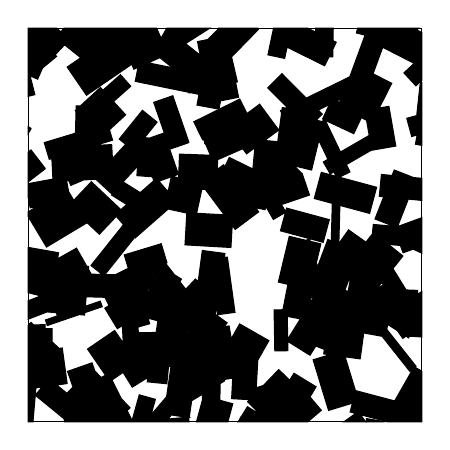
\begin{tikzpicture}[scale=0.01]
\draw[] (0,0) -- (0,500) -- (500,500) -- (500,0) -- (0,0);
\draw[fill=black] (387.3111,484.1532) -- (391.3719,482.1431) -- (387.1578,473.63) -- (387.0131,463.6971) -- (382.275,463.7661) -- (376.6219,452.3461) -- (328.8665,475.9858) -- (325.8316,461.6785) -- (304.6,466.1822) -- (311.7734,500) -- (355.2984,500) -- (365.2604,495.0687) -- (365.3322,500) -- (387.542,500) -- (387.3111,484.1532);
\draw[fill=white] (122.7353,473.2875) -- (123.5583,472.0863) -- (123.1685,472.9651) -- (122.7353,473.2875);
\draw[fill=white] (171.8216,480.3888) -- (175.6589,471.739) -- (179.2104,476.2079) -- (171.8216,480.3888);
\draw[fill=black] (292.7989,498.8186) -- (258.3425,463.5284) -- (265.698,431.9285) -- (263.4617,431.4079) -- (267.2615,412.2854) -- (244.3261,407.728) -- (242.4022,397.2249) -- (214.5027,402.3355) -- (217.0013,415.9756) -- (206.4385,418.1346) -- (204.4783,417.6783) -- (204.2689,418.578) -- (135.975,432.5372) -- (139.6153,450.3473) -- (134.257,447.9702) -- (131.4861,454.216) -- (74.0532,414.8662) -- (49.546,450.6355) -- (66.7878,462.4487) -- (46.2188,478.9721) -- (34.2113,466.2876) -- (35.9778,464.1391) -- (18.8318,450.0411) -- (17.9852,449.1468) -- (11.9414,435.3152) -- (2.314,439.522) -- (8.4067,415.6176) -- (0,413.4749) -- (0,440.5331) -- (0,445.8794) -- (0,448.705) -- (0,459.1366) -- (0,485.1506) -- (0,498.4325) -- (0,500) -- (36.3521,500) -- (41.4372,495.1862) -- (45.3042,500) -- (85.4037,500) -- (102.0631,486.6173) -- (103.5022,487.6033) -- (86.8473,500) -- (163.1215,500) -- (168.7844,487.235) -- (176.0073,500) -- (230.5784,500) -- (199.8832,480.4399) -- (218.6056,465.5608) -- (215.1459,482.9714) -- (228.3846,485.602) -- (242.3778,499.9338) -- (242.3381,500) -- (291.589,500) -- (292.7989,498.8186);
\draw[fill=white] (169.0284,463.3959) -- (152.4127,456.0246) -- (183.5015,449.6702) -- (167.9453,462.033) -- (169.0284,463.3959);
\draw[fill=black] (493.6242,497.8266) -- (500,494.5712) -- (500,450.4912) -- (500,433.6799) -- (492.6361,426.8404) -- (477.4215,443.2215) -- (490.4813,455.3513) -- (450.4512,475.7901) -- (438.0991,442.076) -- (461.8954,430.0032) -- (445.9501,398.5737) -- (458.2839,400.7196) -- (467.0581,350.2882) -- (436.5314,344.9771) -- (436.4633,345.3689) -- (404.3267,326.7595) -- (408.8446,317.3089) -- (395.0669,310.7223) -- (442.6845,297.8969) -- (433.7476,264.7166) -- (395.985,274.8877) -- (394.6736,226.3383) -- (394.7061,226.3261) -- (407.0613,243.7173) -- (429.0629,228.0867) -- (437.3645,238.5011) -- (438.4913,250.6553) -- (464.6641,248.2289) -- (440.6879,257.6311) -- (451.7851,285.9294) -- (446.1493,286.4749) -- (448.8299,314.1673) -- (462.3455,312.859) -- (465.0705,319.8079) -- (489.4909,310.2314) -- (500,309.2141) -- (500,281.2623) -- (482.9574,282.9119) -- (469.2079,247.85) -- (500,259.13) -- (500,239.819) -- (500,214.3475) -- (489.0603,219.3416) -- (476.3475,214.6845) -- (472.9515,223.9547) -- (457.4727,225.3897) -- (476.0707,210.5647) -- (463.338,194.5916) -- (480.1296,167.3879) -- (494.6996,166.8476) -- (494.503,161.5443) -- (500,165.3711) -- (500,143.8639) -- (500,107.7181) -- (484.4434,108.6873) -- (483.1566,106.6922) -- (479.995,108.7314) -- (475.9818,105.9376) -- (469.1819,115.7056) -- (456.7332,123.7347) -- (455.3266,116.0416) -- (456.1227,116.6719) -- (492.7334,70.4297) -- (491.2529,69.2576) -- (500,64.2598) -- (500,45.4311) -- (500,39.9153) -- (500,0) -- (456.0304,0) -- (422.2517,8.9228) -- (428.6056,0) -- (401.3327,0) -- (416.1328,10.5391) -- (409.0367,12.4135) -- (411.9985,23.6257) -- (381.665,14.3602) -- (362.0274,78.6499) -- (383.2434,85.1304) -- (375.5115,86.1891) -- (376.2836,91.8277) -- (365.399,96.232) -- (358.0373,84.4642) -- (329.6957,102.1942) -- (329.9025,90.2632) -- (313.3489,89.9763) -- (312.4465,142.0387) -- (323.6563,142.2329) -- (330.0088,174.5368) -- (317.8668,177.4323) -- (331.7219,235.5321) -- (352.5006,230.5771) -- (357.4829,231.9987) -- (358.2819,229.1984) -- (371.7948,225.9759) -- (366.0616,201.9341) -- (367.6024,196.5341) -- (380.7248,231.5637) -- (385.1333,229.9122) -- (386.388,276.3631) -- (390.9666,276.2394) -- (363.5207,283.6317) -- (372.4576,316.812) -- (391.203,311.7631) -- (388.4335,317.5563) -- (383.7957,314.8707) -- (375.0142,330.0355) -- (380.8516,333.4158) -- (369.2425,357.6994) -- (360.0402,319.8363) -- (338.036,325.1842) -- (347.7742,315.3896) -- (347.9847,315.4614) -- (357.3504,288.0466) -- (321.7504,275.8846) -- (327.0527,266.6897) -- (328.3216,271.3887) -- (382.5646,256.7407) -- (374.787,227.9395) -- (320.544,242.5875) -- (326.845,265.9206) -- (311.4935,257.0681) -- (301.8087,273.863) -- (300.8783,269.44) -- (288.8226,271.9759) -- (292.7837,266.679) -- (263.0076,244.4118) -- (259.1571,249.5607) -- (257.5427,221.417) -- (199.2268,224.762) -- (201.541,265.1073) -- (177.7935,270.3013) -- (135.9054,233.5539) -- (135.2224,234.3325) -- (97.4821,186.9871) -- (110.3539,186.6463) -- (127.2222,194.8851) -- (122.0645,211.9142) -- (168.9556,226.1164) -- (176.2173,202.1406) -- (174.2437,201.5428) -- (185.7918,186.7145) -- (194.6452,181.1368) -- (192.6286,177.9358) -- (200.1875,168.23) -- (212.4501,181.2742) -- (216.0018,177.9353) -- (221.2304,217.5276) -- (249.9357,213.7367) -- (249.2529,208.5666) -- (253.0159,209.0859) -- (262.6866,139.0087) -- (240.8534,135.9957) -- (239.9987,142.1888) -- (237.4744,139.5036) -- (238.2407,138.3597) -- (236.6403,137.2876) -- (252.6589,125.6576) -- (249.0099,120.6316) -- (255.2371,121.6703) -- (257.9554,105.3737) -- (268.6826,124.1797) -- (305.7904,103.013) -- (291.6788,78.2736) -- (289.7271,43.1641) -- (298.6973,45.9086) -- (318.3224,66.1719) -- (332.2958,52.6385) -- (337.708,61.5124) -- (365.7997,44.3791) -- (357.9293,31.4748) -- (372.3743,14.5064) -- (355.3338,0) -- (266.7424,0) -- (269.5968,4.588) -- (269.5458,5.7699) -- (270.3539,5.8048) -- (278.5706,19.0118) -- (290.5099,11.5837) -- (289.5106,14.8502) -- (278.7296,25.2916) -- (281.4112,28.0604) -- (258.4502,29.3368) -- (259.9012,55.4398) -- (259.8107,55.4914) -- (248.401,53.5882) -- (249.4403,51.8635) -- (241.6744,47.1836) -- (243.7935,47.1512) -- (243.4882,27.2381) -- (259.8674,22.7818) -- (253.669,0) -- (213.8993,0) -- (221.188,26.7893) -- (221.3125,34.9133) -- (207.6459,26.6777) -- (204.5091,5.2376) -- (203.756,5.3478) -- (204.2536,0) -- (46.1651,0) -- (45.6069,3.682) -- (9.0462,33.606) -- (17.6725,44.1455) -- (9.692,43.0479) -- (6.0515,0) -- (0,0) -- (0,41.715) -- (0,84.9183) -- (0,87.7093) -- (0,122.4154) -- (3.4582,126.1658) -- (7.1075,122.8008) -- (21.3066,123.4353) -- (21.5438,118.1259) -- (30.2845,118.071) -- (30.1807,101.5249) -- (39.3014,93.1146) -- (43.2075,93.6518) -- (49.4159,48.5113) -- (36.1587,46.688) -- (48.9856,36.1895) -- (56.9966,43.847) -- (49.9762,63.9169) -- (81.0034,74.7701) -- (84.6042,64.4759) -- (92.5708,56.1415) -- (98.2583,58.9728) -- (75.4147,92.3164) -- (109.7735,115.8555) -- (120.818,99.7343) -- (119.6298,122.1751) -- (113.2244,118.2762) -- (97.3851,144.2984) -- (102.7113,147.5404) -- (97.5368,158.1346) -- (73.5503,158.7698) -- (72.5346,146.6406) -- (91.5643,153.1688) -- (93.967,146.1649) -- (71.8597,138.581) -- (71.6066,135.559) -- (64.7295,136.1349) -- (24.2697,122.2551) -- (21.867,129.2589) -- (37.3425,134.5678) -- (35.406,138.5906) -- (23.9107,139.5532) -- (3.5527e-15,130.2836) -- (0,153.6529) -- (16.0858,159.8889) -- (0,163.9769) -- (0,193.8621) -- (0,221.4645) -- (38.5895,214.6499) -- (37.2106,206.8415) -- (61.3487,220.4931) -- (74.3708,197.4682) -- (76.7742,197.267) -- (76.4789,193.7407) -- (79.9939,187.5256) -- (79.8666,187.4536) -- (94.1571,187.0752) -- (79.8018,198.5181) -- (121.1433,250.3812) -- (111.8448,260.9805) -- (90.3948,238.2472) -- (74.8283,252.935) -- (23.2536,221.9848) -- (0,260.7342) -- (0,266.7001) -- (11.1845,273.412) -- (2.4655,271.8024) -- (0,285.1583) -- (0,302.4679) -- (31.3893,308.2625) -- (30.0644,334.4337) -- (26.786,333.442) -- (20.385,354.6025) -- (60.0842,366.6115) -- (60.7427,394.2247) -- (59.8072,395.2395) -- (60.7885,396.1442) -- (60.9117,401.3085) -- (66.2522,401.1812) -- (91.7645,424.7009) -- (94.9945,421.1973) -- (117.1729,440.9265) -- (130.2049,426.2767) -- (108.2867,406.779) -- (123.7747,389.9788) -- (103.164,370.9778) -- (107.1635,357.7561) -- (88.9161,352.2363) -- (88.8918,351.2168) -- (106.0193,352.0839) -- (106.9273,334.1496) -- (123.8413,352.474) -- (115.6388,359.0832) -- (145.092,395.6368) -- (163.6948,380.6476) -- (147.7452,360.853) -- (154.1326,360.3586) -- (172.457,366.7889) -- (190.8424,314.3962) -- (183.0788,311.6718) -- (191.1516,309.9062) -- (192.2488,339.9953) -- (231.6485,338.5587) -- (225.5159,352.6108) -- (224.0616,353.6003) -- (224.6845,354.5159) -- (222.7919,358.8528) -- (221.6809,358.3024) -- (210.4014,381.0701) -- (268.7954,409.9995) -- (277.9622,391.4963) -- (294.0412,403.3879) -- (318.2884,370.6024) -- (300.3343,357.3241) -- (317.0883,355.7717) -- (321.9823,392.2456) -- (320.5472,395.1827) -- (322.5047,396.1392) -- (322.898,399.07) -- (327.2953,398.48) -- (329.1788,399.4002) -- (304.4073,424.2976) -- (322.3921,442.1914) -- (353.2599,411.1668) -- (408.6391,438.2262) -- (428.0458,491.1954) -- (417.0071,494.0478) -- (418.5451,500) -- (495.821,500) -- (493.6242,497.8266);
\draw[fill=white] (397.9061,410.4182) -- (391.9081,407.4875) -- (395.5521,405.7782) -- (397.9061,410.4182);
\draw[fill=white] (382.6779,402.9774) -- (368.3657,395.9842) -- (373.5508,390.7727) -- (365.8897,383.1504) -- (372.7697,381.4783) -- (376.6943,383.3545) -- (374.0545,384.5927) -- (382.6779,402.9774);
\draw[fill=black] (3.7361,372.5916) -- (0,366.3506) -- (0,374.8282) -- (3.7361,372.5916);
\draw[fill=white] (423.2712,386.4219) -- (413.6925,366.0004) -- (377.4374,383.0059) -- (396.7448,342.6191) -- (433.2626,363.7654) -- (429.9064,383.0557) -- (423.2712,386.4219);
\draw[fill=black] (500,431.6688) -- (500,390.6623) -- (500,378.0109) -- (500,372.854) -- (500,353.033) -- (500,351.1763) -- (492.0577,352.6254) -- (494.1923,364.3245) -- (487.3087,362.4555) -- (481.0474,385.5164) -- (493.6843,388.9475) -- (498.2914,431.8523) -- (500,431.6688);
\draw[fill=white] (141.1758,352.6999) -- (139.709,350.8794) -- (140.9465,349.7372) -- (141.1758,352.6999);
\draw[fill=black] (204.2693,354.7451) -- (180.0978,346.3689) -- (159.5106,405.7782) -- (183.6821,414.1544) -- (204.2693,354.7451);
\draw[fill=white] (287.9914,348.1957) -- (277.467,340.4121) -- (272.6486,346.9272) -- (240.6987,332.9837) -- (240.2459,320.5662) -- (248.0958,326.4365) -- (249.8472,324.0945) -- (255.5455,335.7245) -- (285.4769,321.0591) -- (287.9914,348.1957);
\draw[fill=black] (21.7524,321.5537) -- (0,304.825) -- (0,342.5711) -- (3.5119,345.2719) -- (21.7524,321.5537);
\draw[fill=white] (85.9827,308.0962) -- (70.6835,307.3216) -- (54.0771,300.3347) -- (51.5451,306.3527) -- (48.7524,306.2113) -- (51.3514,292.1324) -- (57.8776,281.2574) -- (80.1772,304.8912) -- (117.7303,269.458) -- (125.2018,276.0125) -- (105.9918,288.0312) -- (107.9163,291.1072) -- (106.2933,289.3488) -- (85.9827,308.0962);
\draw[fill=white] (181.8515,311.2412) -- (165.9414,305.6581) -- (177.6991,292.2555) -- (181.8515,311.2412);
\draw[fill=white] (139.0163,324.8005) -- (120.4695,304.7072) -- (142.3245,291.0338) -- (159.6144,306.2018) -- (157.8597,311.2022) -- (138.0822,312.7331) -- (139.0163,324.8005);
\draw[fill=white] (220.5699,295.2606) -- (213.9182,264.8479) -- (249.2402,262.8218) -- (225.1054,295.0952) -- (220.5699,295.2606);
\draw[fill=white] (157.8214,189.9842) -- (162.3705,180.6704) -- (163.5799,182.5901) -- (157.8214,189.9842);
\draw[fill=white] (407.1643,179.9889) -- (402.3268,167.0754) -- (406.4935,165.3894) -- (408.7296,177.6196) -- (410.5554,177.2858) -- (407.1643,179.9889);
\draw[fill=white] (449.2914,176.97) -- (444.5838,171.0643) -- (446.1182,170.7838) -- (451.254,173.7904) -- (449.2914,176.97);
\draw[fill=white] (155.5116,169.7835) -- (150.9659,167.5633) -- (152.5123,165.0227) -- (155.5116,169.7835);
\draw[fill=white] (16.7228,159.727) -- (16.9291,159.1949) -- (16.9684,159.6646) -- (16.7228,159.727);
\draw[fill=white] (359.6353,158.9095) -- (357.836,149.7596) -- (362.0871,156.555) -- (359.6353,158.9095);
\draw[fill=white] (44.437,137.8343) -- (38.4181,134.9368) -- (46.3879,137.6709) -- (44.437,137.8343);
\draw[fill=white] (152.2952,131.5534) -- (154.3027,124.5158) -- (139.4896,120.2904) -- (139.8755,113.0008) -- (162.6068,113.3769) -- (164.71,128.2603) -- (152.2952,131.5534);
\draw[fill=white] (202.6611,114.5244) -- (200.8602,113.3179) -- (200.8944,111.2518) -- (203.3311,113.8945) -- (202.6611,114.5244);
\draw[fill=white] (329.1457,133.926) -- (329.6521,104.7074) -- (345.873,130.6366) -- (329.1457,133.926);
\draw[fill=white] (426.3054,112.8081) -- (421.7925,79.8516) -- (402.6348,82.475) -- (415.9923,38.7451) -- (416.1763,39.4414) -- (465.6402,26.3754) -- (489.223,67.6505) -- (484.7995,64.1483) -- (449.6547,108.539) -- (426.3054,112.8081);
\draw[fill=white] (178.346,71.0295) -- (176.0872,48.2427) -- (151.2948,50.7002) -- (151.8357,56.1566) -- (132.1839,43.9613) -- (120.5388,62.7264) -- (106.3502,53.0059) -- (118.0675,29.4676) -- (129.3358,17.6792) -- (125.6769,14.1817) -- (132.0008,1.4779) -- (141.0959,34.1357) -- (161.5666,28.4347) -- (156.0241,8.533) -- (175.87,31.7889) -- (181.3493,69.2398) -- (178.346,71.0295);
\draw[fill=white] (181.8836,8.5478) -- (177.466,3.3712) -- (201.7951,5.6347) -- (181.8836,8.5478);
\draw[fill=black] (452.9025,0) -- (429.206,0) -- (429.8737,3.9215) -- (452.9025,0);
\end{tikzpicture}
}}%
\vspace*{-10pt}%
\label{fig:booleanModel}%
\end{figure}

\vspace*{-18pt}

\section{Simulation of a 2-D Boo\-lean model}
\vspace*{-10pt}
\index{Spatial Processes!Characterization}
Let $\{x_i;i\in \mathbb{N}\}$ be a random collection of points in $\mathbb{R}^2$ forming a stationary Poisson point process with intensity $\gamma>0$. 
Let $Z_0,Z_1,Z_2,\dots$ be independent, identically distributed random 2-D convex bodies (nonempty, compact, convex sets) with distribution $\mathbb{Q}$, which are independent of the point process $\{x_i;i\in \mathbb{N}\}$. The random points $x_1,x_2,\dots$ are the germs and the random sets $Z_1,Z_2,\dots$ are the grains of the Boolean
model. The random set $Z_0$ is called the typical grain. The union of the translated grains:\vspace*{-8pt}
\begin{eqnarray}
Z=\bigcup_{i=1}^{\infty}(Z_i+x_i)
\end{eqnarray}
\vspace*{-12pt}

\noindent is a random closed set, which is called the stationary Boolean model with intensity $\lambda$ and grain distribution $\mathbb{Q}$. The random collection $X=\{Z_1+x_1,Z_2+x_2,\dots\} $ of the shifted grains is the particle process underlying the Boolean model. 

Figure \ref{fig:booleanModel} shows a realization of two different Boolean models $Z$ observed in a compact and convex observation window $W$.


\textls[-20]{We are going to simulate some realizations of a Boolean model of 2-D disks in a squared observation window. The final simulated model will be represented as a discrete binary image.}

\begin{qbox}
\begin{itemize}
\item
Generate a 2-D discrete observation window $W$ of size $500 \times 500$.
\item
Generate the random germs that follows a Poisson law with intensity $\lambda=100/(500*500)$. Take care of the edge effects (a grain with a germ outside the observation window could intersect it!)
\item Generate the random grains (as disks). The disk radius will follow a uniform distribution $\mathcal{U}(10,50)$.
\item Vizualize the realization.
\end{itemize}
\end{qbox}

\begin{mcomment}
\begin{mremark}
 Look at the \matlabregistered{} function \minline{poissrnd} and \minline{randi}.
 
 The \minline{meshgrid} function can be used to generate the disks.
\end{mremark}
\end{mcomment}

\begin{pcomment}
\begin{premark}
 Look at the \pinline{numpy} functions \minline{random.poisson} and \minline{random.randint}.
 
 Use \pinline{skimage.draw.circle} to generate the disks in an array.
\end{premark}
\end{pcomment}
\vspace*{-8pt}
\section{Geometrical characterization of a 2-D Boo\-lean mo\-del}\vspace*{-8pt}

Assume we observe $Z$ in a compact, convex observation window $W$ with positive volume (as shown in Figure \ref{fig:booleanModel}).
Our aim is to extract distributional information from the geometric properties of the sample $Z \cap W$. Thus, we assume we can measure geometric functionals like the perimeter of the sample $Z \cap W$ which is a finite union of convex bodies (a polyconvex set). By a geometric functional $\phi$ we mean a real-valued functional defined on the space of polyconvex sets with specific additional properties. Important examples of geometric functionals are the Minkowski functionals $W_{\nu}$ that are related in the 2-D space to the measures of area ($A$), perimeter ($P$) and Euler number ($\chi$):
\begin{eqnarray}
W_0&=&A\\
W_1&=&P/2\\
W_2&=&\pi \chi
\end{eqnarray}
%
The boundary of the observation window $W$ has a disturbing effect. It is therefore of advantage to assume a sufficiently large observation
window and to consider only limits as the window tends to infinity. This motivates the introduction of the density (or specific value) of the Boolean model for a geometric functional $\phi$. The density of $\phi$ is the combined spatial and probabilistic mean value:\vspace*{-8pt}
\begin{eqnarray}
\overline{\phi}(Z)=\lim_{r\rightarrow\infty}\frac{\mathbb{E}[\phi(Z\cap rW)]}{W_0(rW)}
\end{eqnarray}
The crucial problem when studying a Boolean model is, that the particles overlap and can therefore not be observed individually.

For this purpose, the Miles formula gives relationships between the global Minkowski densities and the Minkowski densities of the particle.\index{Spatial Processes!Miles Formula}
For isotropic Boolean models and by using the densities of the particle process $X$:
\begin{eqnarray}
\overline{\phi}(X)=\gamma\mathbb{E}[\phi(Z_0)]
\end{eqnarray}
Miles formulas express the observable Minkowski densities $\overline{W}_{\nu}(Z)$ in terms of the Minkowski densities $\overline{W}_{\nu}(X)$ and can be inverted.\\
For example in 2-D: \vspace*{-8pt}
\begin{eqnarray}
\overline{W}_0(Z)&=&1-e^{-\overline{W}_0(X)}\\
\overline{W}_1(Z)&=&e^{-\overline{W}_0(X)}\overline{W}_1(X)\label{eq:miles2}\\
\overline{W}_2(Z)&=&e^{-\overline{W}_0(X)}\left(\overline{W}_2(X)-\overline{W}_1(X)^2\right)\label{eq:miles3}
\end{eqnarray}
\vspace*{-8pt}
\begin{qbox}
\begin{itemize}
\item Generate different realizations of the previous Boolean model and compute the Minkowski densities of $Z$ (by using the functions done in the tutorial "Integral Geometry").
\item Compute the theoretical Minkowski densities of $Z$ by using the Miles formulas.
\item Compare the computed and theoretical values. 
\end{itemize}
\end{qbox}
